\chapter{\altGerEng{Auswertung}{Evaluation}}


Many numerical results can be used to analyze the influence of critical factors on system performance. Key parameters analyzed include channel gain and pulse response \cite{fan2017circuit}, data rate\cite{liu2016visible}, and harvested energy\cite{diamantoulakis2018simultaneous}.

Since light irradiance affects the data transferred and also the energy harvested, it is essential to evaluate the effect of distance and the angle between the transmitter and receiver \cite{fong2012integrated}. 

According to the paper, \cite{mahmoud2022design}, increasing the distance allows the light's intensity to be lowered, and noise and delays are increased. The effect of increasing distance on the generated voltage was shown in this paper, along with the effect of angle of incidence.

In this chapter of the thesis, the prototype will be evaluated. The evaluation can be broken down into two sections: i)Communication Module Evaluation, ii)Energy Harvesting Evaluation. Charging and discharging times will also be evaluated to check the capability of energy harvesting. 

\section{Communication Module}

The communication module's waveform and pulse gain were evaluated to determine the response against the sent signal. Next, an Eye diagram to assess the effectiveness of the \ac{VLC} system's communication. Finally, decoded data from STM32 is evaluated to see if this module can achieve one of the primary goals of the thesis.


\subsection{Waveform and Pulse Gain}

In paper \cite{fan2017circuit}, the pseudo-random bit sequence of the transmitter, receiver amplifier output, and final output from the comparator are compared side by side to understand the performance of the \ac{VLC} system. Input and output of the transmitter and receiver are essential for knowing the performance of the communication branch \cite{tudose2011energy}.

An example \ac{UART} signal is sent from the transmitter to the receiver, as shown in Figure \ref{fig:5.1}. The \ac{PD} receives this signal, and it generates a photo current that is amplified by the \ac{TIA} shown in Figure \ref{fig:5.2}. There is noise, and spikes are visible. At the output of the comparator, the noise is reduced \ref{fig:5.3}, and the construction of the \ac{UART} is firm but inverted. It is inverted because the \ac{OPAmp} was in inverting mode and the comparator was in non-inverting mode. With the same baud rate, the amplifier's responses are shown at 10 and 15 cm distance in Figure \ref{fig:5.4} and Figure \ref{fig:5.5}, respectively. Noises are much more prominent than before, and increase with distance.

\begin{figure}
    \centering
    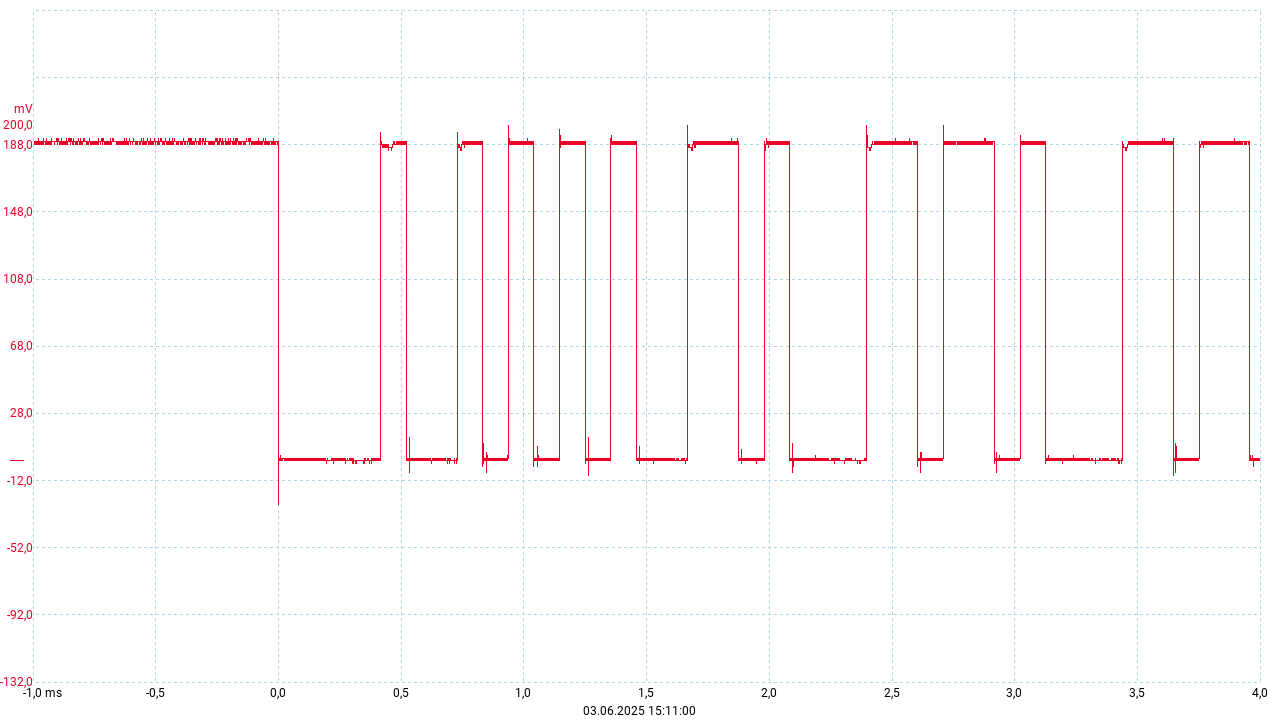
\includegraphics[width=0.75\linewidth]{fig/transmitter_UART_9600.png}
    \caption{UART signal sent from transmitter}
    \label{fig:5.1}
\end{figure}



\begin{figure}[ht]
    \centering
    \begin{minipage}[b]{0.45\linewidth}
        \centering
        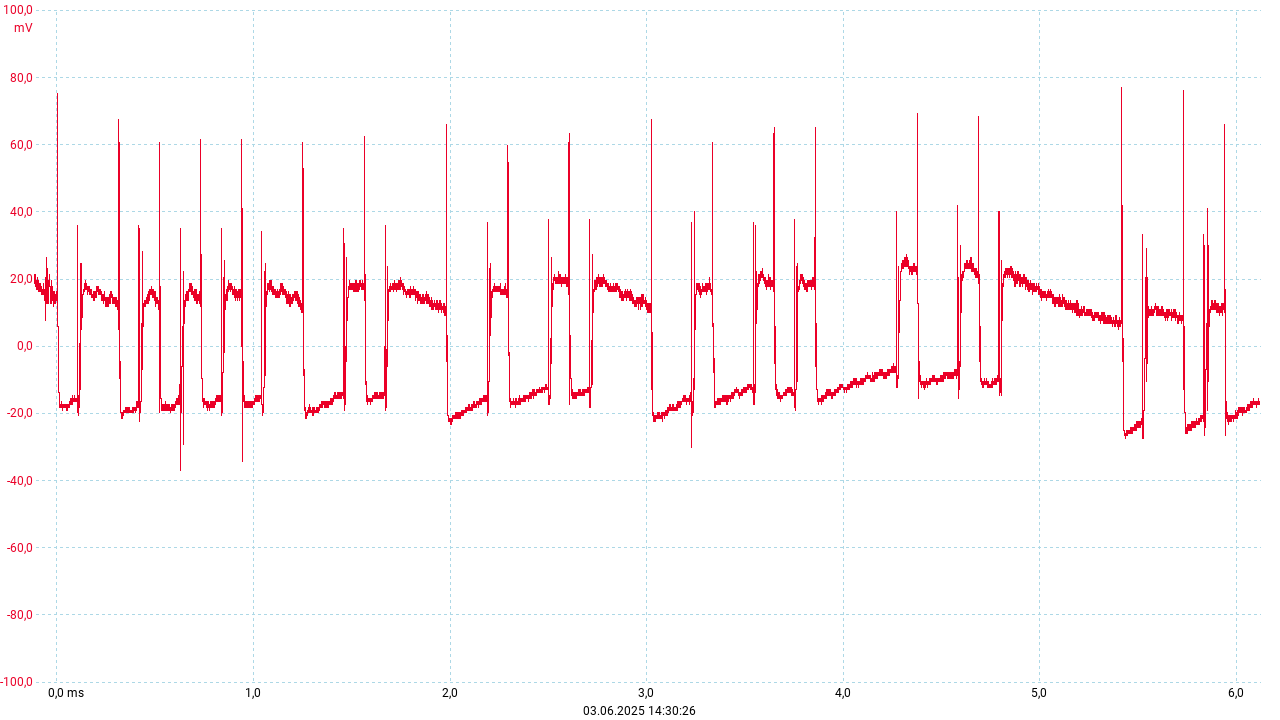
\includegraphics[width=\linewidth]{fig/amplifier_UART_9600.png}
        \caption{Amplifier output with 9600 baud rate at 5cm distance}
        \label{fig:5.2}
    \end{minipage}
    \hspace{0.05\linewidth} % Adjust horizontal space between images
    \begin{minipage}[b]{0.45\linewidth}
        \centering
        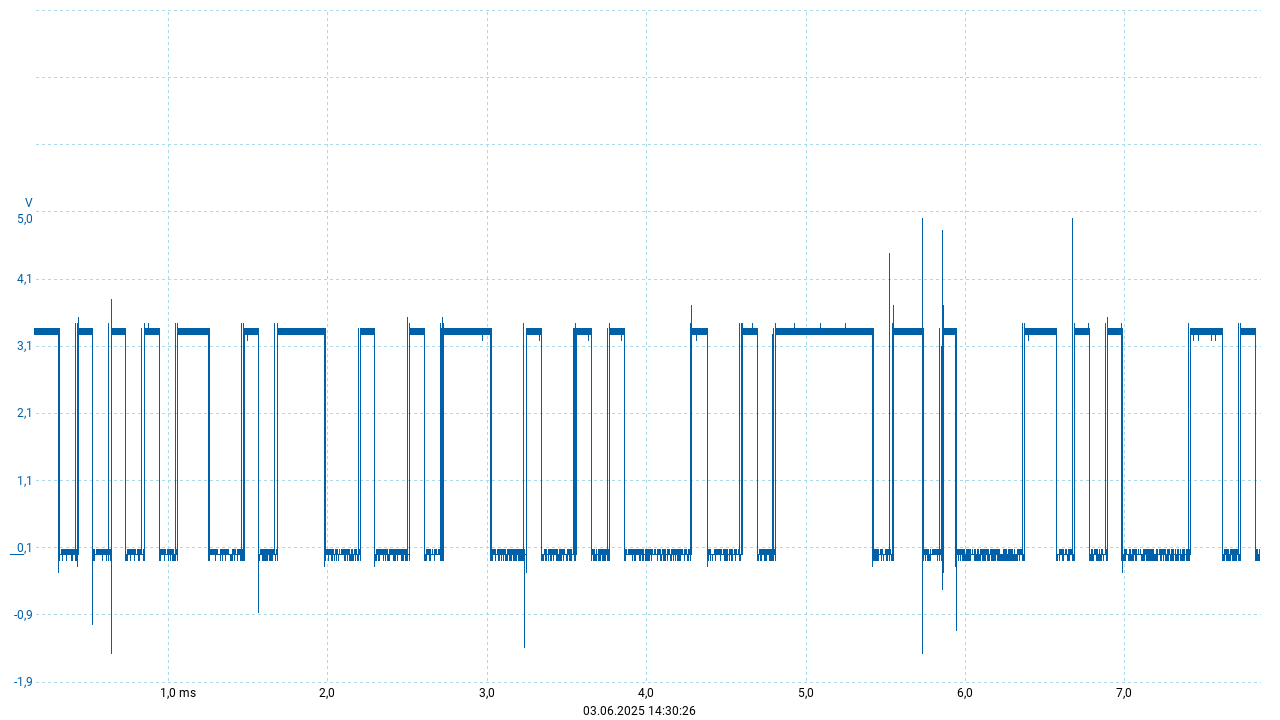
\includegraphics[width=\linewidth]{fig/comparator_UART_9600.png}
        \caption{Comparator output with 9600 baud rate at 5cm distance}
        \label{fig:5.3}
    \end{minipage}
\end{figure}

\begin{figure}[ht]
    \centering
    \begin{minipage}[b]{0.45\linewidth}
        \centering
        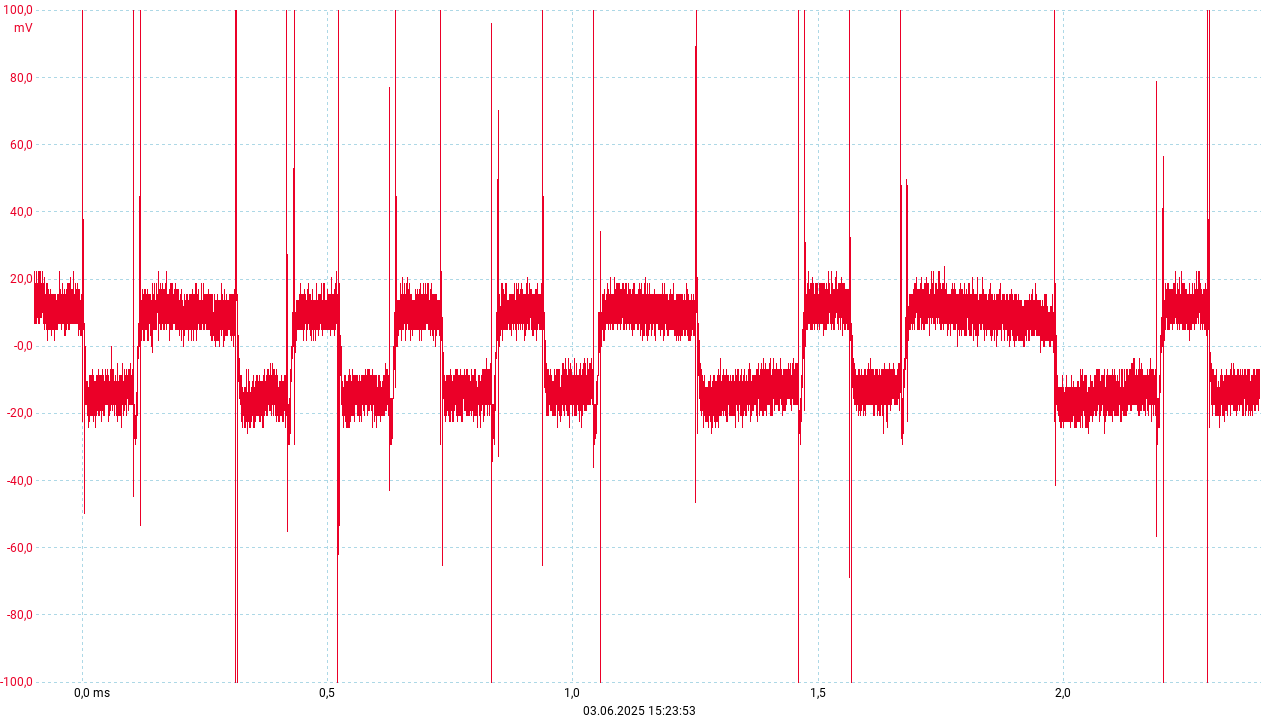
\includegraphics[width=\linewidth]{fig/amplifier_UART_9600_10cm.png}
        \caption{Amplifier output with 9600 baud rate at 10cm distance}
        \label{fig:5.4}
    \end{minipage}
    \hspace{0.05\linewidth} % Adjust horizontal space between images
    \begin{minipage}[b]{0.45\linewidth}
        \centering
        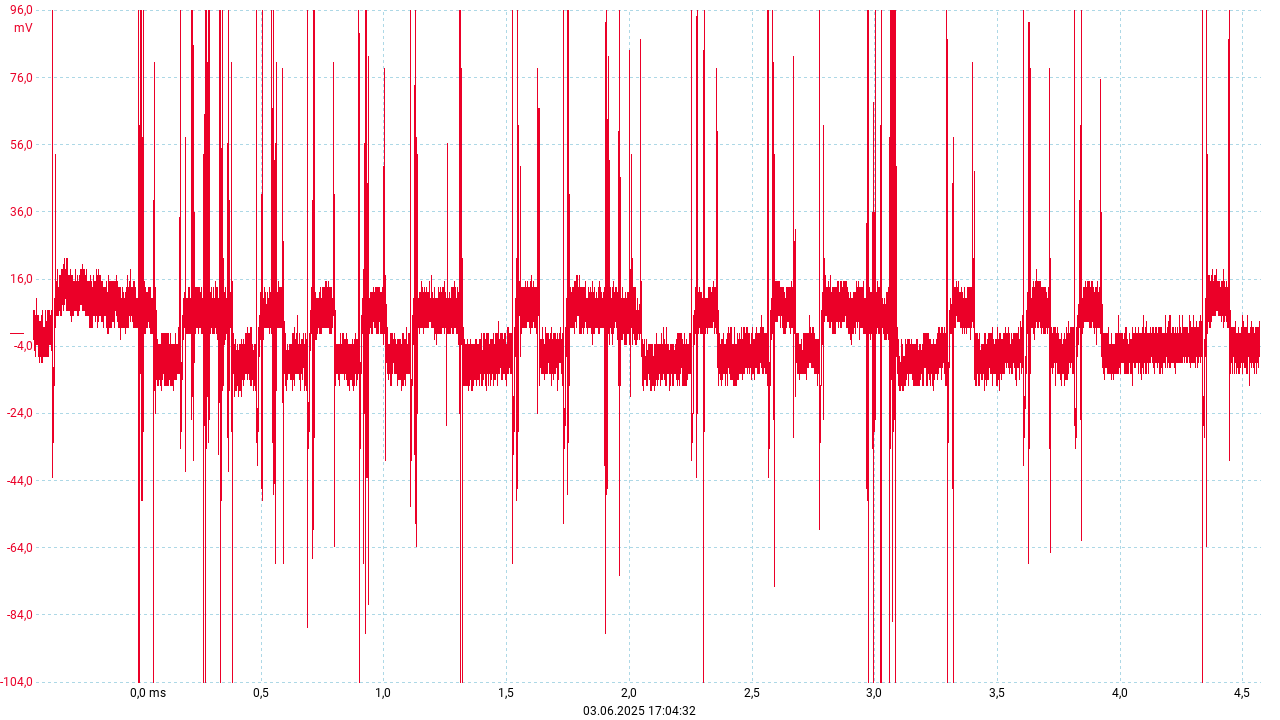
\includegraphics[width=\linewidth]{fig/amplifier_UART_9600_15cm.png}
        \caption{Amplifier output with 9600 baud rate at 15cm distance}
        \label{fig:5.5}
    \end{minipage}
\end{figure}


Output responses from the comparator at distances 10 and 15cm are shown compared to the original \ac{UART} signal at 4800 baud rate from the pico in Figure \ref{fig:5.6} and Figure \ref{fig:5.7}. It is visible that with the distance, more noise is added, indicating that a 4800 baud rate is unsuitable for long distances. Figure \ref{fig:5.8} and Figure \ref{fig:5.9} show signal response at baud rate 9600 at 10 and 15 cm. This baud rate is suitable for both distances. The same is visible at a baud rate of 14400 and 19200 in Figures \ref{fig:5.10}, \ref{fig:5.11}, \ref{fig:5.12}, and \ref{fig:5.13}. This indicates that with increasing distances, a higher baud rate performs well. More waveforms showcasing the comparator Output vs the original UART with different baud rates at various distances are shown in \ref{appendix:A3}.

\begin{figure}[ht]
    \centering
    \begin{minipage}[b]{0.45\linewidth}
        \centering
        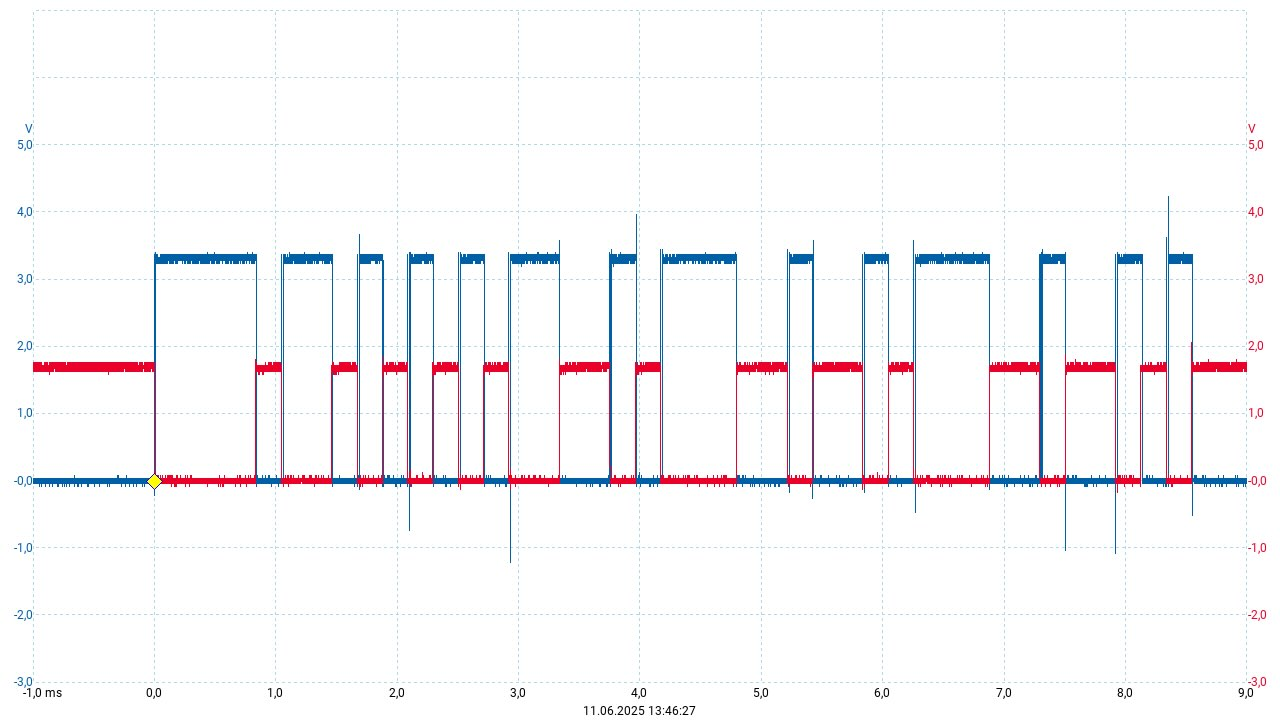
\includegraphics[width=\linewidth]{fig/compvs/comp vs original 10cm 4800.jpg}
        \caption{Output vs original UART with 4800 baud rate at 10cm distance}
        \label{fig:5.6}
    \end{minipage}
    \hspace{0.05\linewidth} % Adjust horizontal space between images
    \begin{minipage}[b]{0.45\linewidth}
        \centering
        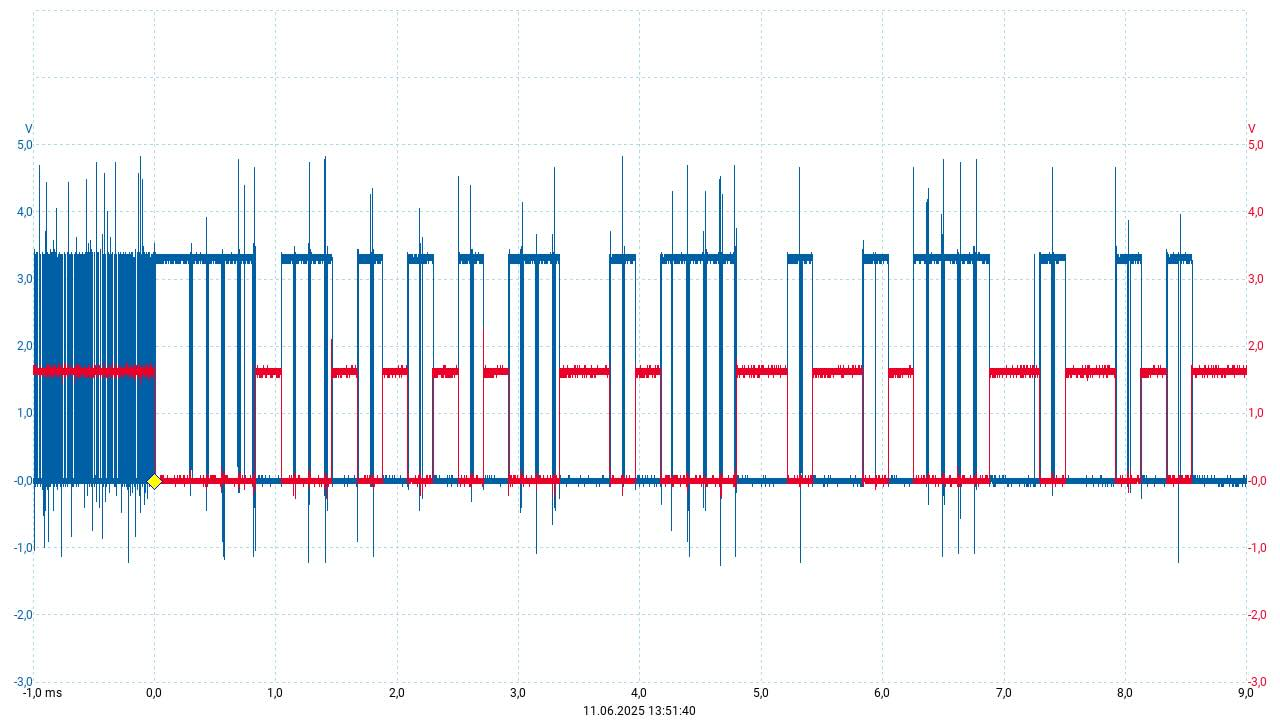
\includegraphics[width=\linewidth]{fig/compvs/comp vs original 15cm 4800.jpg}
        \caption{Output vs original UART with 4800 baud rate at 15cm distance}
        \label{fig:5.7}
    \end{minipage}
\end{figure}

\begin{figure}[ht]
    \centering
    \begin{minipage}[b]{0.45\linewidth}
        \centering
        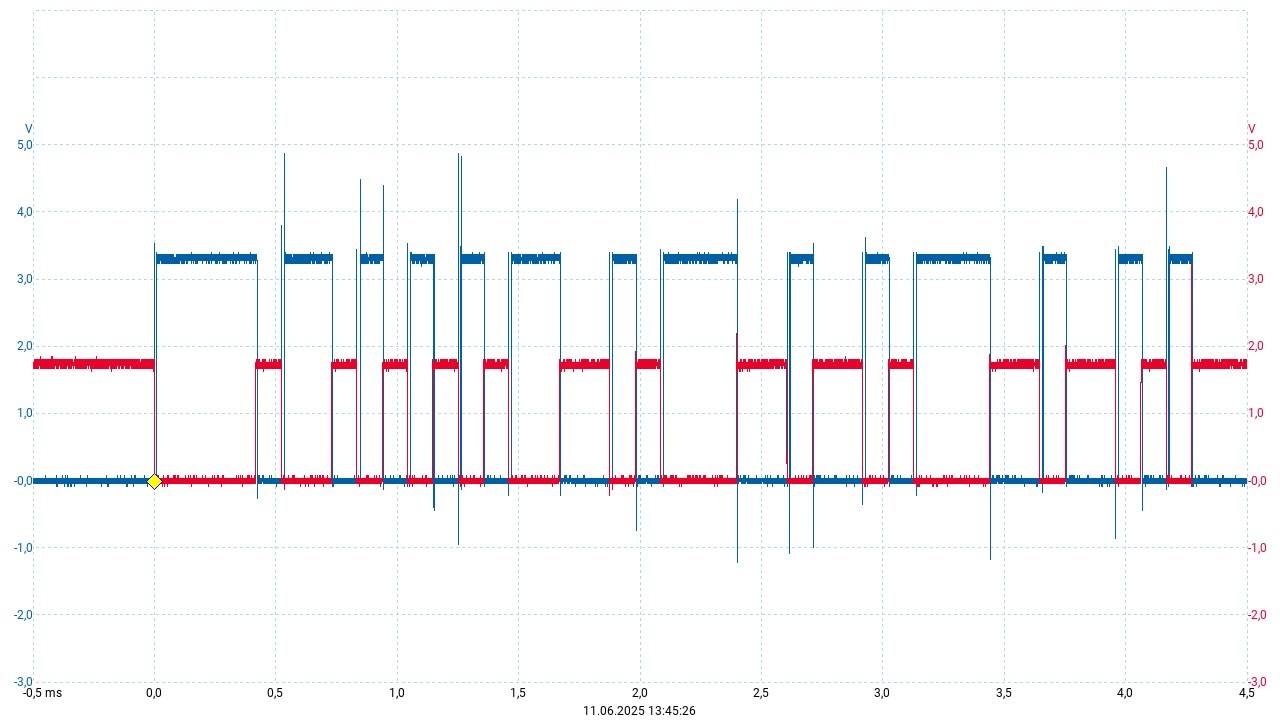
\includegraphics[width=\linewidth]{fig/compvs/comp vs original 10cm 9600.jpg}
        \caption{Output vs original 9600 baud rate at 10cm}
        \label{fig:5.8}
    \end{minipage}
    \hspace{0.05\linewidth} % Adjust horizontal space between images
    \begin{minipage}[b]{0.45\linewidth}
        \centering
        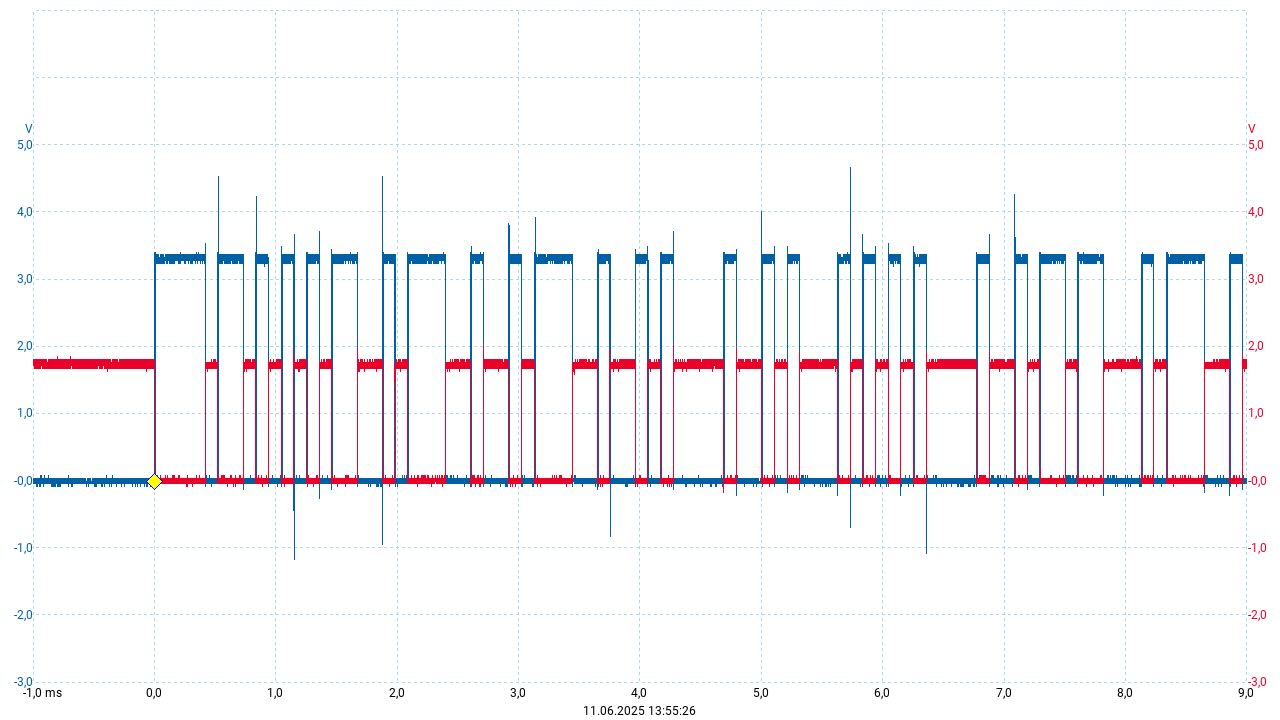
\includegraphics[width=\linewidth]{fig/compvs/comp vs original 15cm 9600-0002.jpg}
        \caption{Output vs original 9600 baud rate at 15cm}
        \label{fig:5.9}
    \end{minipage}
\end{figure}

\begin{figure}[ht]
    \centering
    \begin{minipage}[b]{0.45\linewidth}
        \centering
        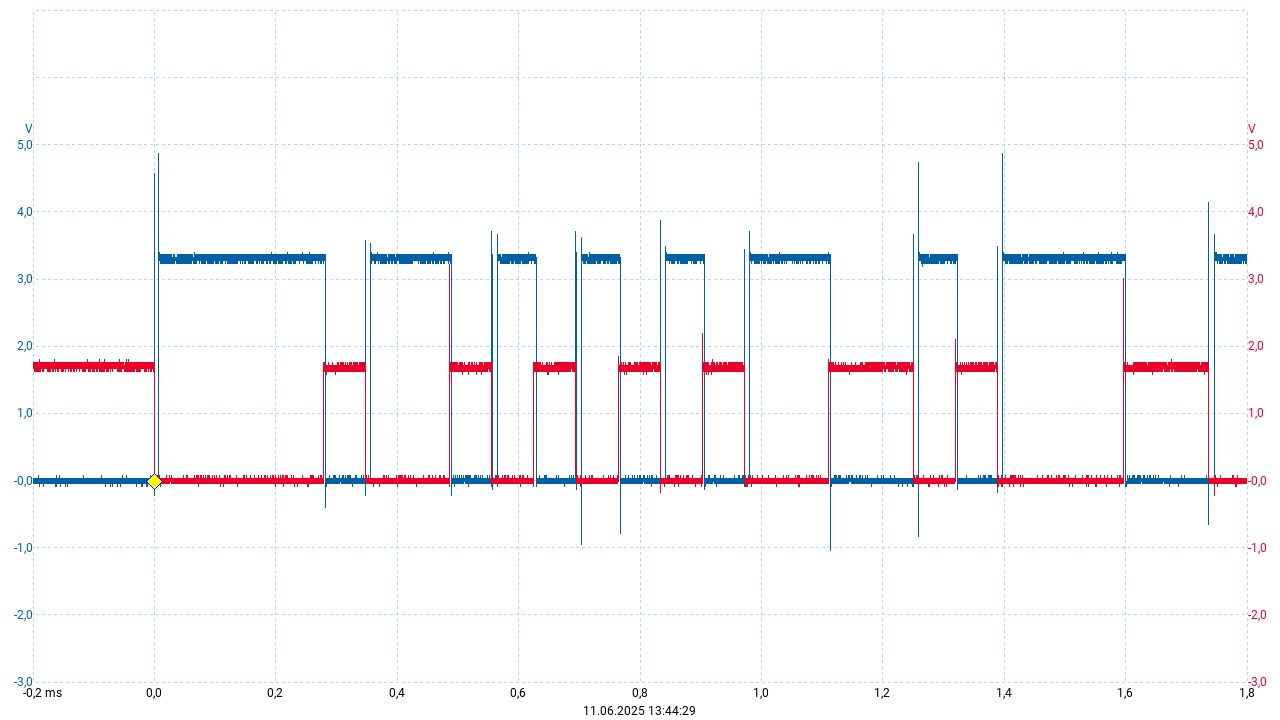
\includegraphics[width=\linewidth]{fig/compvs/comp vs original 10cm 14400.jpg}
        \caption{Output vs original 14400 baud rate at 10cm.}
        \label{fig:5.10}
    \end{minipage}
    \hspace{0.05\linewidth} % Adjust horizontal space between images
    \begin{minipage}[b]{0.45\linewidth}
        \centering
        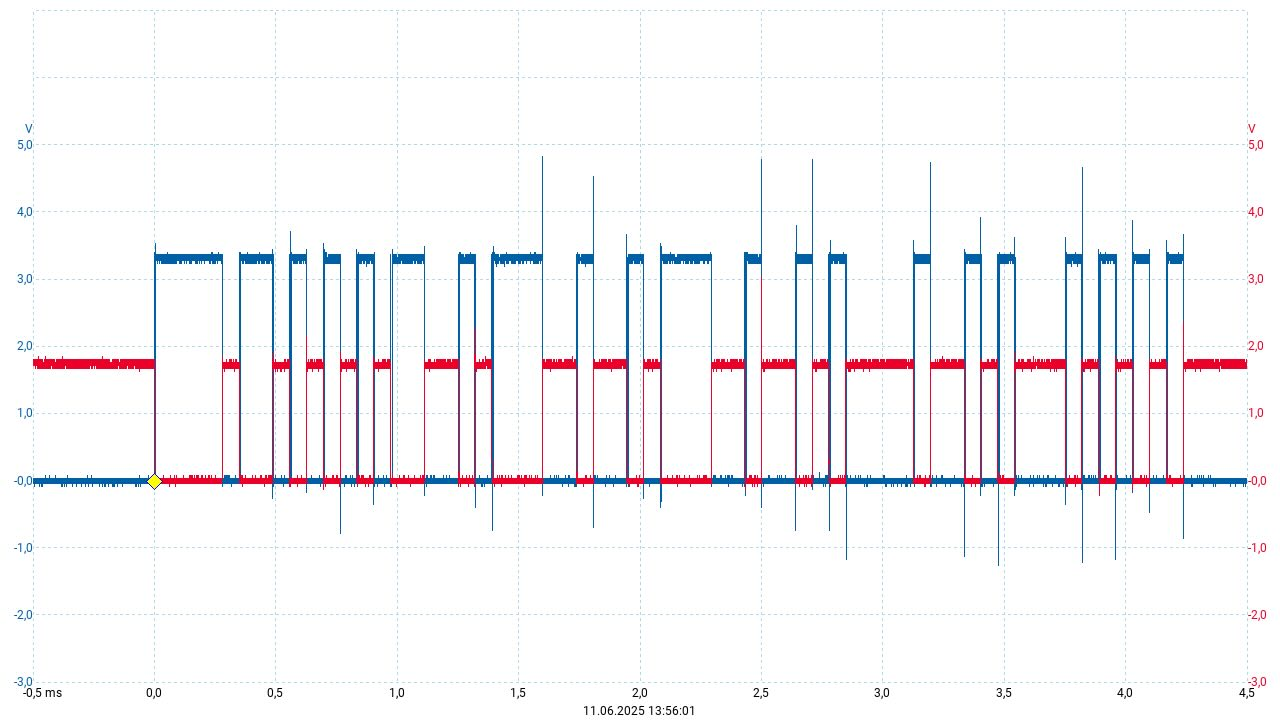
\includegraphics[width=\linewidth]{fig/compvs/comp vs original 15cm 14400.jpg}
        \caption{Output vs original 14400 baud rate at 15cm.}
        \label{fig:5.11}
    \end{minipage}
\end{figure}

\begin{figure}[ht]
    \centering
    \begin{minipage}[b]{0.45\linewidth}
        \centering
        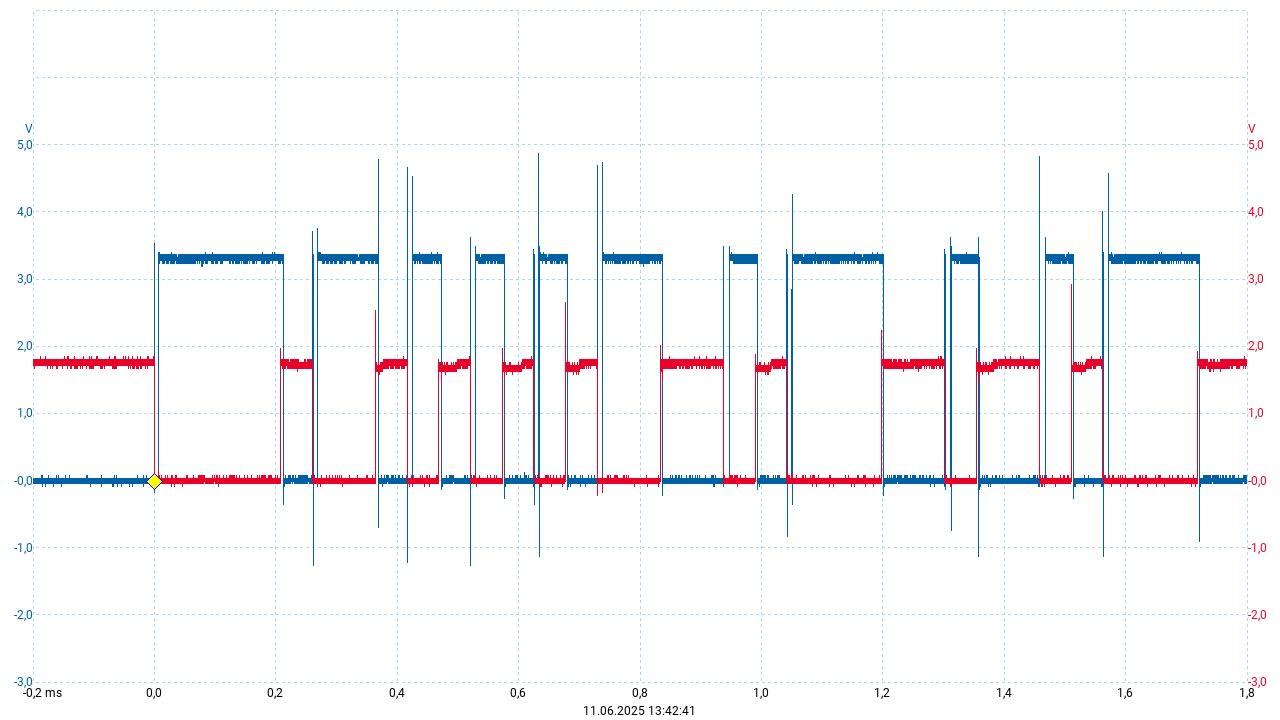
\includegraphics[width=\linewidth]{fig/compvs/comp vs original 10cm 19200.jpg}
        \caption{Output vs original 19200 baud rate at 10cm.}
        \label{fig:5.12}
    \end{minipage}
    \hspace{0.05\linewidth} % Adjust horizontal space between images
    \begin{minipage}[b]{0.45\linewidth}
        \centering
        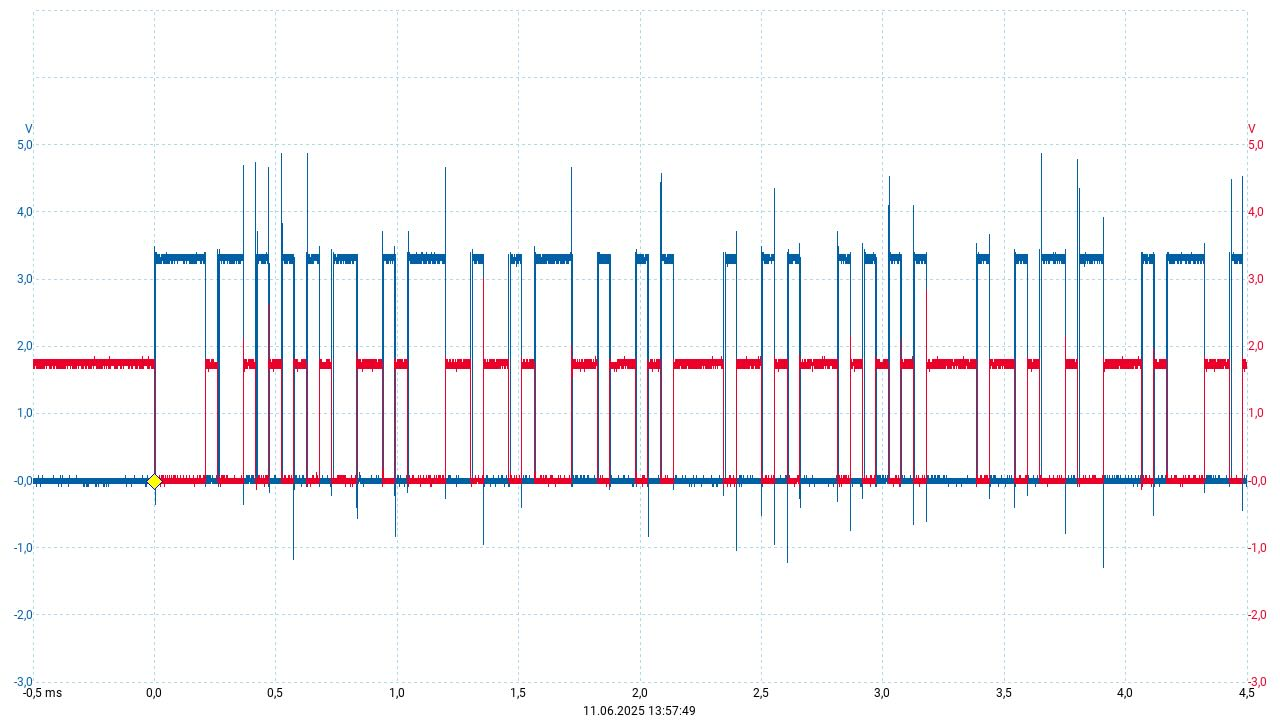
\includegraphics[width=\linewidth]{fig/compvs/comp vs original 15cm 19200.jpg}
        \caption{Output vs original 19200 baud rate at 15cm.}
        \label{fig:5.13}
    \end{minipage}
\end{figure}


\subsection{Eye diagram}
An Eye diagram indicates how noise might impact system performance visually. The eye diagram is a helpful measurement or simulation for channel compliance\cite{Shin:16}\cite{wang2022high}. The measurement shows many factors that can simultaneously affect signal behavior, ultimately allowing for the qualification of errors and losses in a channel \cite{eye_2022}. Identifying variances that can lead to bit error rates is crucial in this measurement. By overlaying signal traces, statistics can be taken at various points along the time domain measurements \cite{eye_2022}.

This process involves overlaying a bitstream's rising and falling edges within a time-domain sampling trace, such as that displayed on an oscilloscope. A signal integrity simulator can also perform a similar superposition of signal levels. Combining the rising and falling edges makes it easier to visualize the variance in signal behavior \cite{eye_2022} \cite{eye_2023}.

Figures in \ref{fig:5.14} show the eye diagrams when the baud rate is set to 9600 at different distances. These are digital signal eye diagrams where lower and higher levels represent the response at 0 and 1, respectively. Ideally, two crossings of an eye diagram should represent the transition between high and low. In the Figure \ref{fig:5.14}, at a 5cm distance, much jitter is seen during crossing, indicating much noise. This is also seen at 10 cm. At 15 cm, the jitter is less, and the crossings are much more prominent. This means the 9600 baud rate has better signal intensity at 15 cm distance. In the case of a 5-LED configuration, multiple responses are seen in the inner eye diagram, which indicates poor signal quality and larger BER. As shown in the Figure \ref{fig:5.15}, the eye diagram response at baud rate 14400 during 2-LED configuration is similar, indicating similar signal integrity. However, for a 5-LED configuration, the response is much worse as the center of the eye is not even visible. As shown in the Figure \ref{fig:5.16}, the eye diagram response at baud rate 19200 during 2-LED configuration has much jitter at 5cm, which gradually improves if the distance increases. With 5 LEDs, there is now a visible crossing in the middle of the eye diagram, indicating this will produce false responses. 

\begin{figure}[t]
    \centering
    
    % First row of subfigures
    \begin{subfigure}[t]{0.48\textwidth}
        \centering
        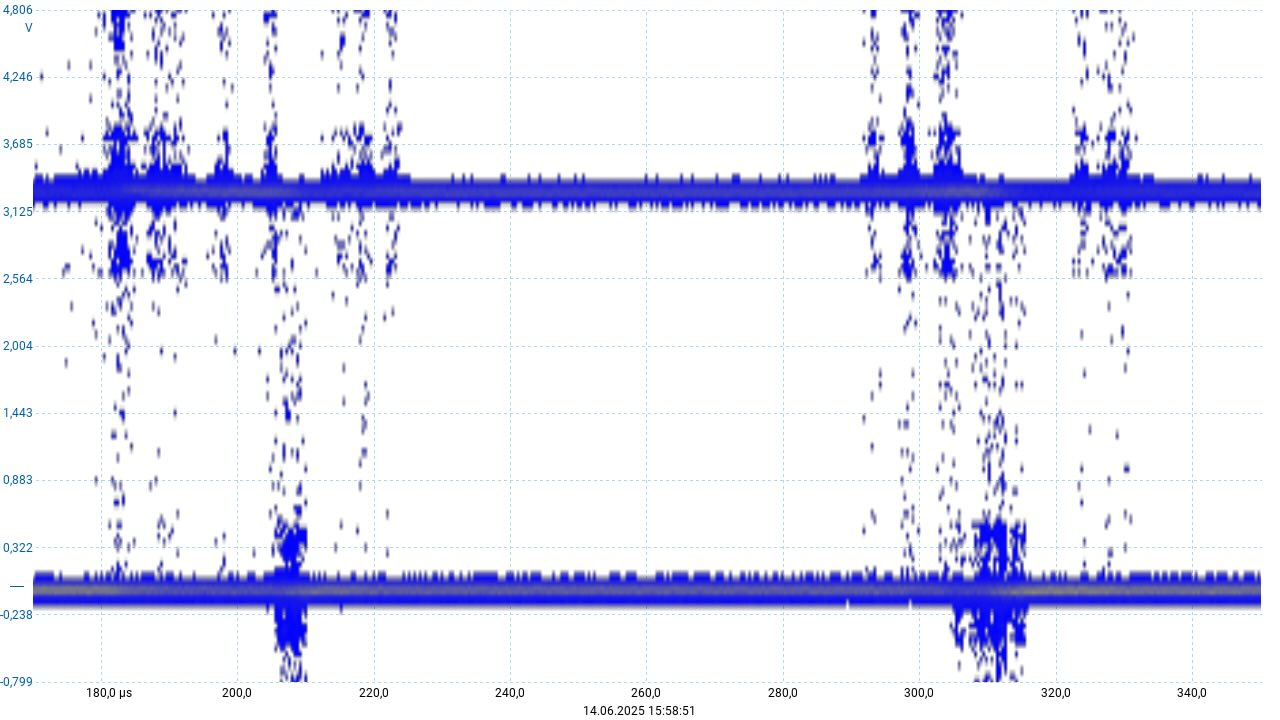
\includegraphics[width=1\textwidth]{fig/eye/eye_9600_5cm_002-0002-zoom.jpg}
        \caption{Two-LEDs at 5cm}
        \label{fig:5.14-a}
    \end{subfigure}
    \hfill
    \begin{subfigure}[t]{0.48\textwidth}
        \centering
        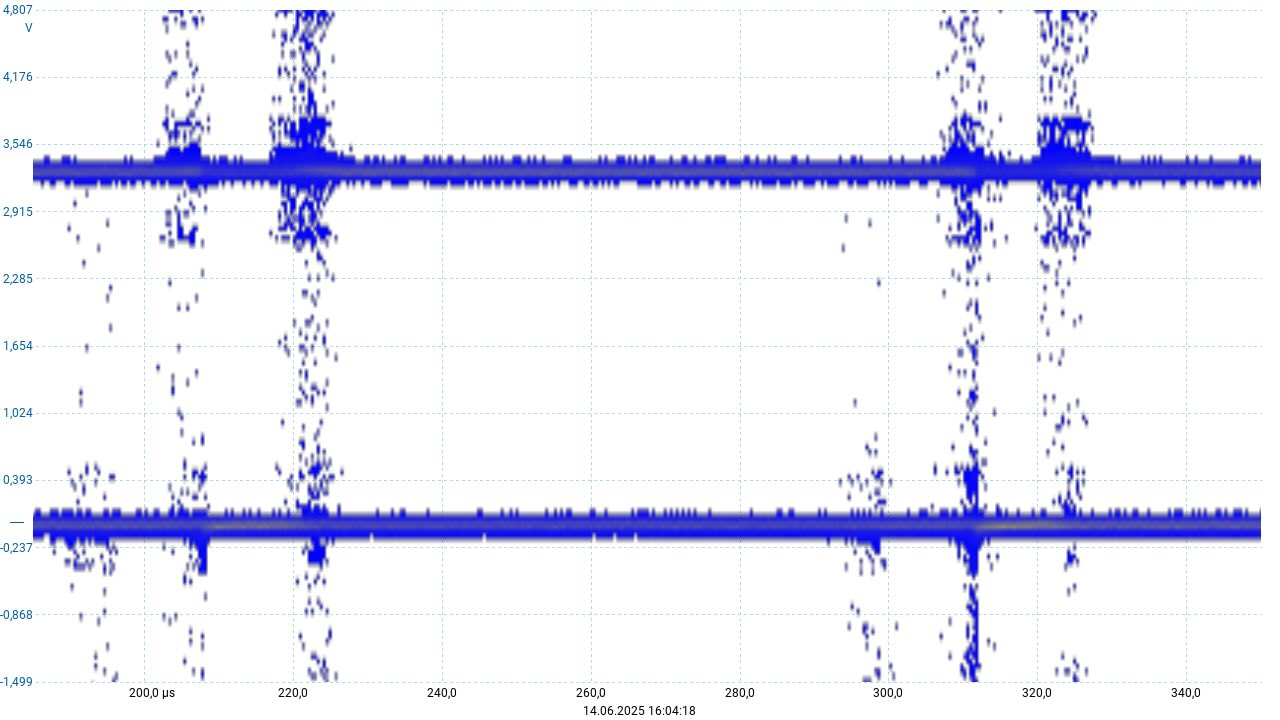
\includegraphics[width=1\textwidth]{fig/eye/eye_9600_10cm-zoom.jpg}
        \caption{Two-LEDs at 10cm}
        \label{fig:5.14-b}
    \end{subfigure}
    
    \vspace{0.5em} % Small vertical space between rows

    % Second row of subfigures
    \begin{subfigure}[t]{0.48\textwidth}
        \centering
        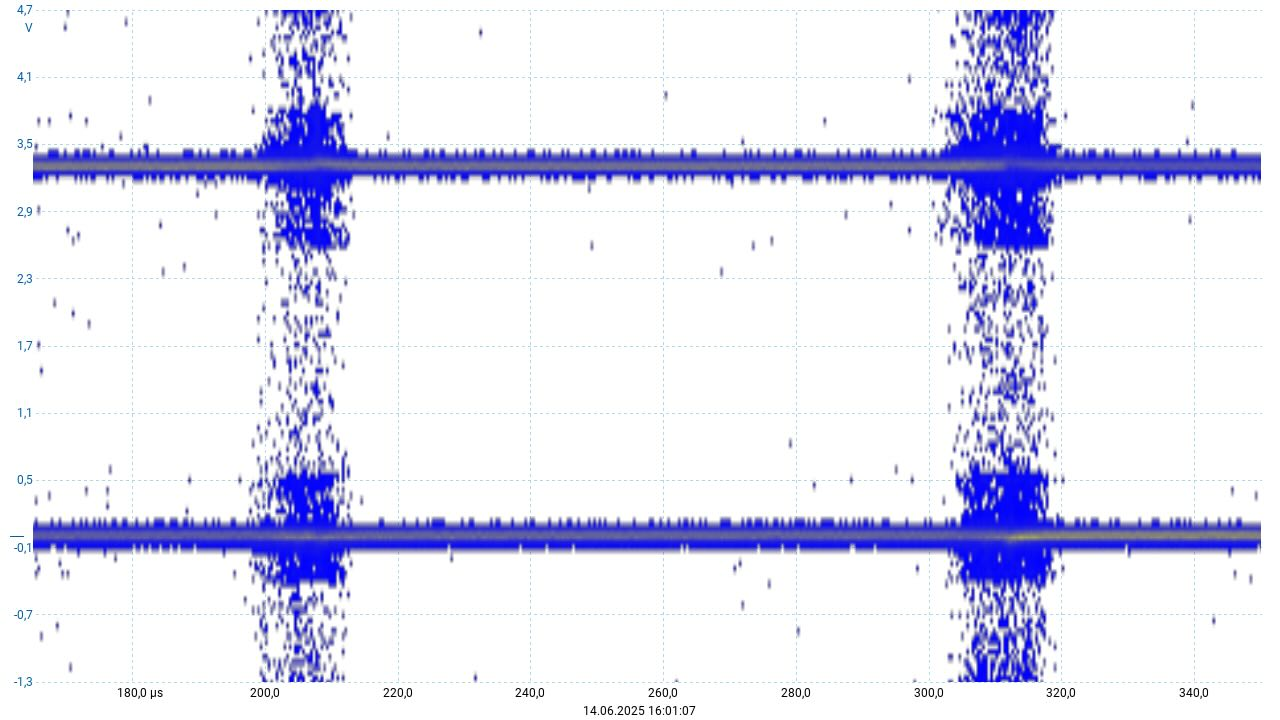
\includegraphics[width=1\textwidth]{fig/eye/eye_9600_15cm-zoom.jpg}
        \caption{Two-LEDs at 15cm}
        \label{fig:5.14-c}
    \end{subfigure}
    \hfill
    \begin{subfigure}[t]{0.48\textwidth}
        \centering
        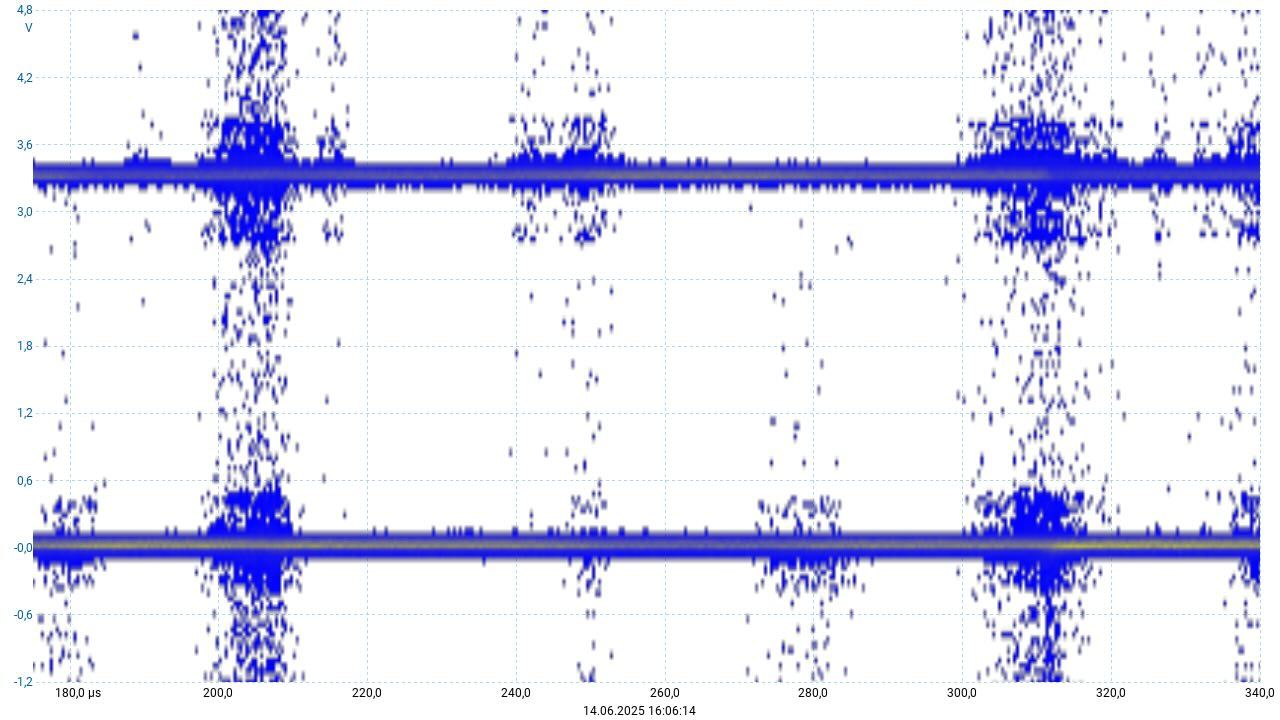
\includegraphics[width=1\textwidth]{fig/eye/eye_9600_5Led_15cm-zoom.jpg}
        \caption{Five-LEDs at 15cm}
        \label{fig:5.14-d}
    \end{subfigure}

    \caption{Eye diagram of 9600 baud rate at different distances and configurations}
    \label{fig:5.14}
\end{figure}




\begin{figure}[t]
    \centering
    
    % First row of subfigures
    \begin{subfigure}[t]{0.48\textwidth}
        \centering
        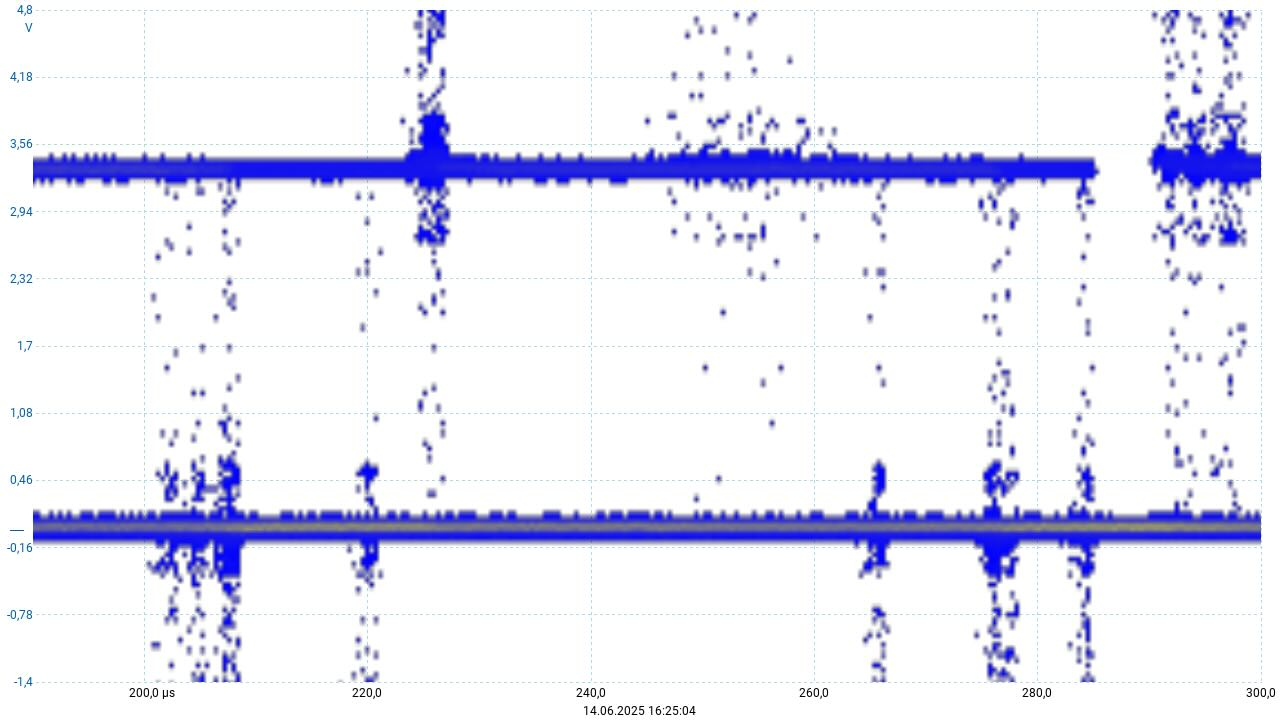
\includegraphics[width=1\textwidth]{fig/eye/eye_14400_5cm_002-zoom.jpg}
        \caption{Two-LEDs at 5cm}
        \label{fig:5.15-a}
    \end{subfigure}
    \hfill
    \begin{subfigure}[t]{0.48\textwidth}
        \centering
        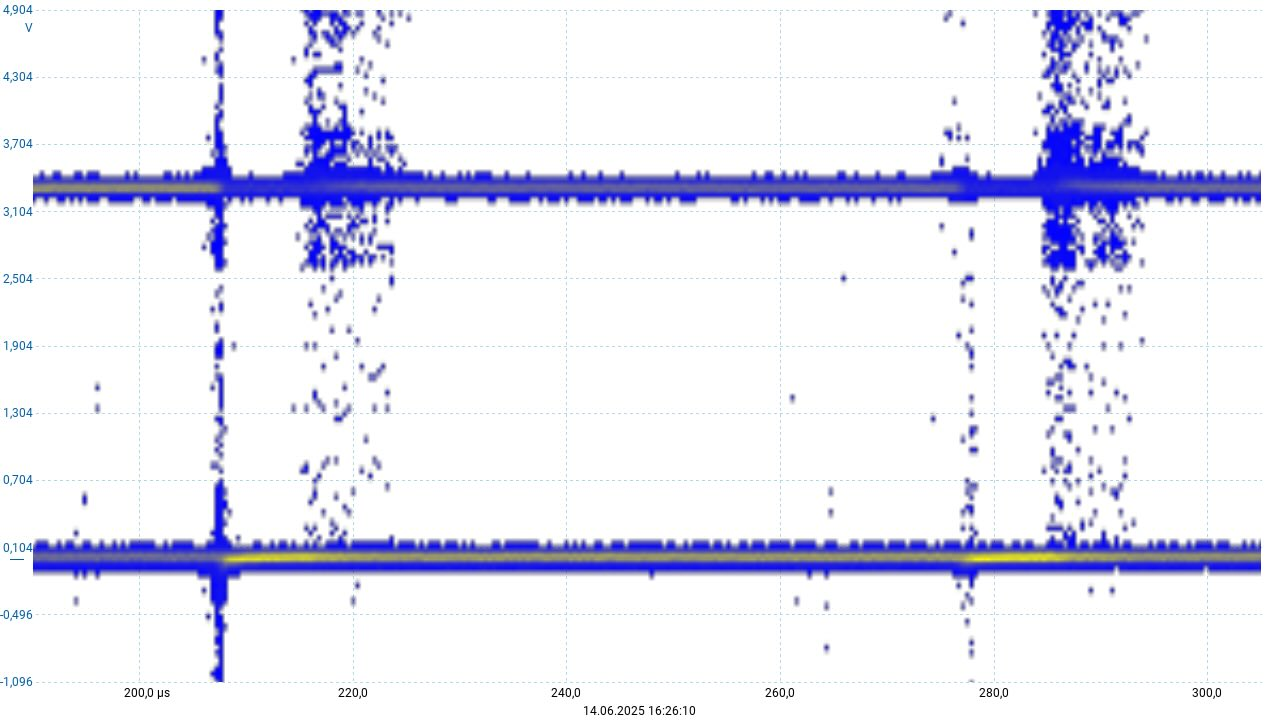
\includegraphics[width=1\textwidth]{fig/eye/eye_14400_10cm-zoom.jpg}
        \caption{Two-LEDs at 10cm}
        \label{fig:5.15-b}
    \end{subfigure}
    
    \vspace{0.5em} % Small vertical space between rows

    % Second row of subfigures
    \begin{subfigure}[t]{0.48\textwidth}
        \centering
        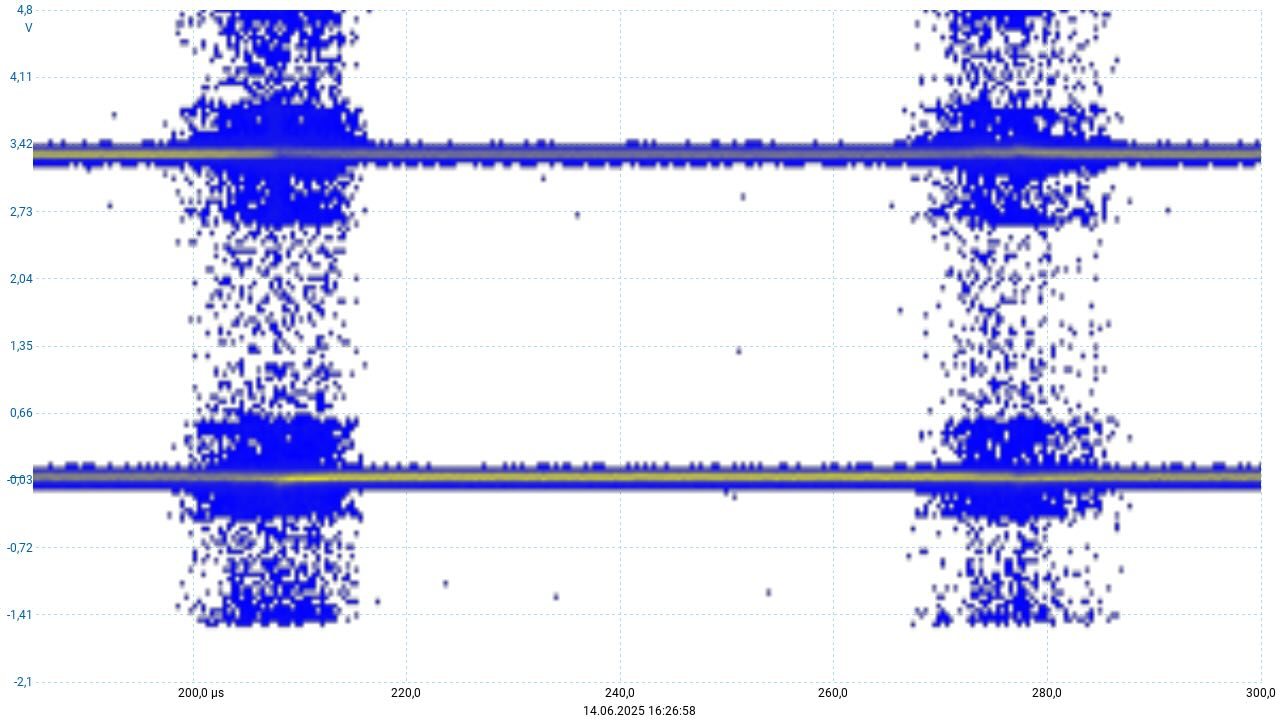
\includegraphics[width=1\textwidth]{fig/eye/eye_14400_15cm-zoom.jpg}
        \caption{Two-LEDs at 15cm}
        \label{fig:5.15-c}
    \end{subfigure}
    \hfill
    \begin{subfigure}[t]{0.48\textwidth}
        \centering
        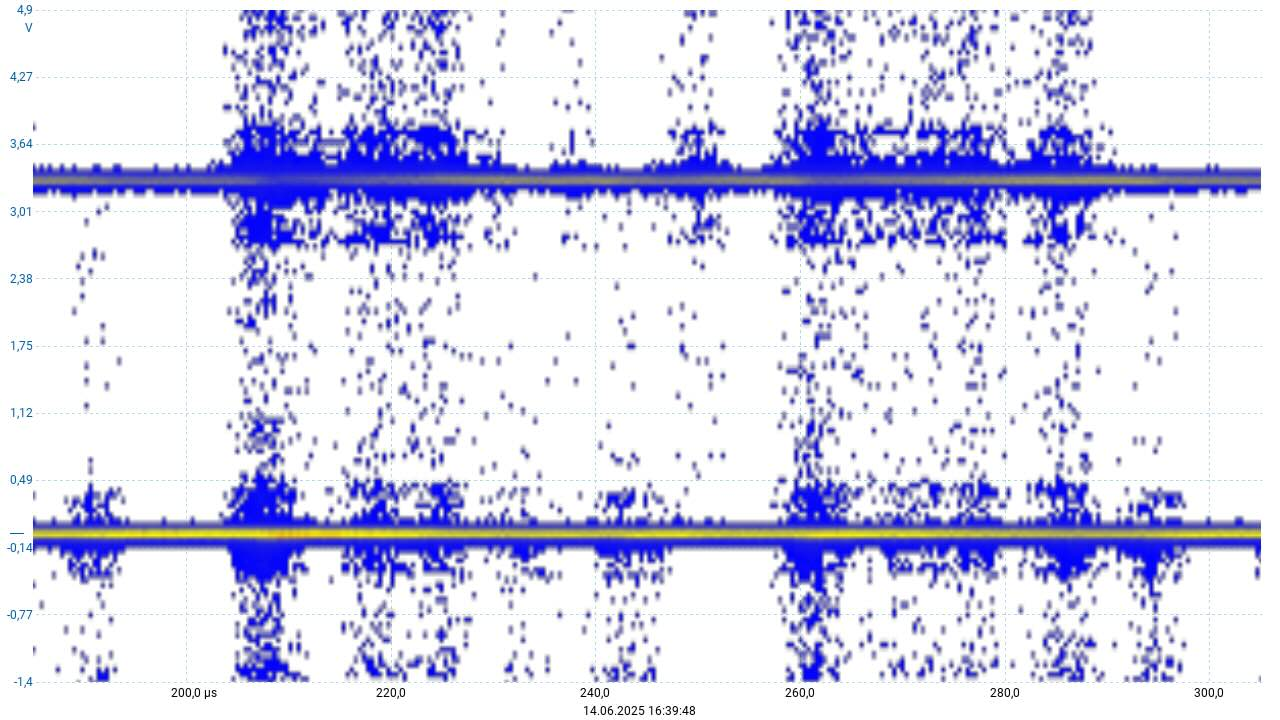
\includegraphics[width=1\textwidth]{fig/eye/eye_14400_5Led_15cm-zoom.jpg}
        \caption{Five-LEDs at 15cm}
        \label{fig:5.15-d}
    \end{subfigure}

    \caption{Eye diagram of 14400 baud rate at different distances and configurations}
    \label{fig:5.15}
\end{figure}




\begin{figure}[t]
    \centering
    
    % First row of subfigures
    \begin{subfigure}[t]{0.48\textwidth}
        \centering
        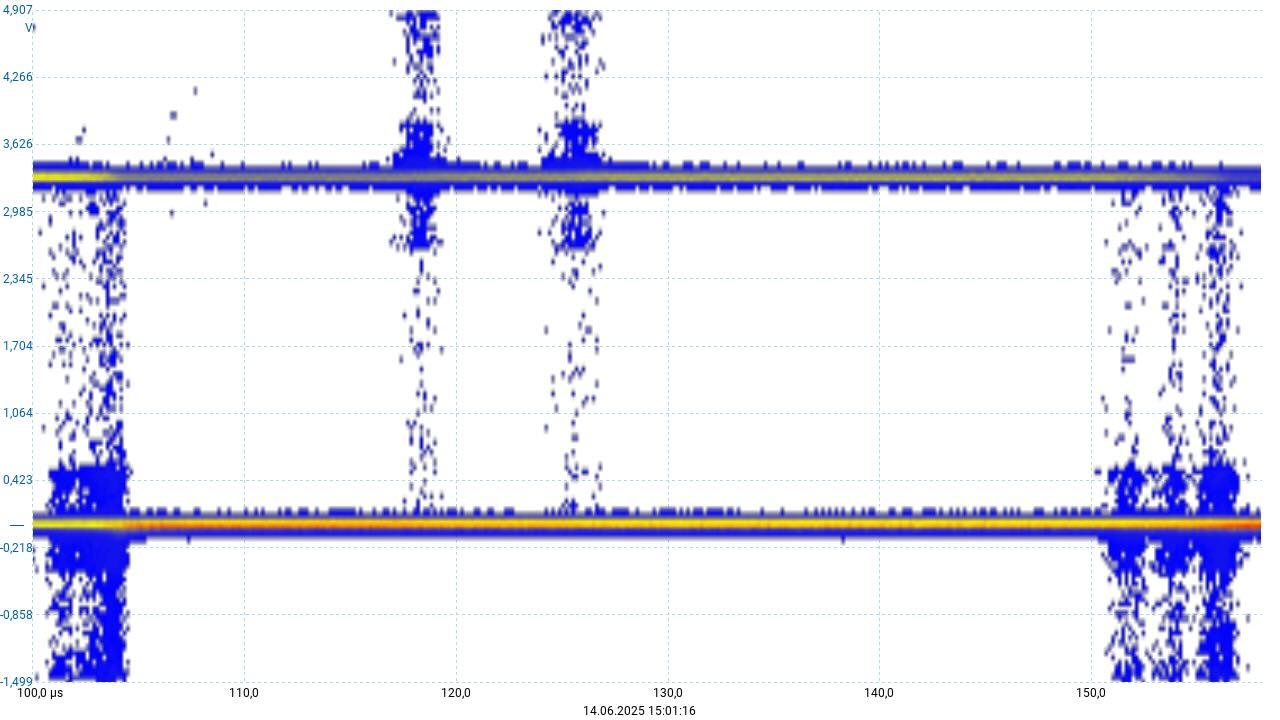
\includegraphics[width=1\textwidth]{fig/eye/eye_19200-zoom.jpg}
        \caption{Two-LEDs at 5cm}
        \label{fig:5.16-a}
    \end{subfigure}
    \hfill
    \begin{subfigure}[t]{0.48\textwidth}
        \centering
        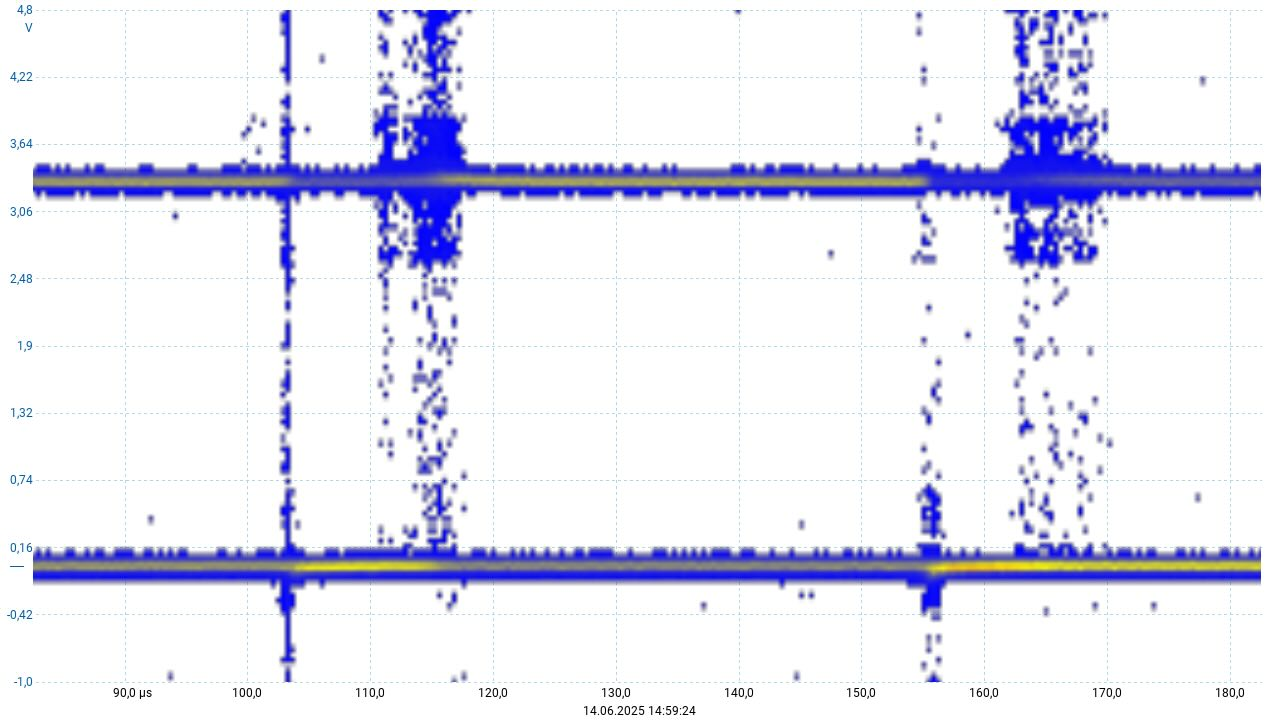
\includegraphics[width=1\textwidth]{fig/eye/eye_19200_10cm_zoom.jpg}
        \caption{Two-LEDs at 10cm}
        \label{fig:5.16-b}
    \end{subfigure}
    
    \vspace{0.5em} % Small vertical space between rows

    % Second row of subfigures
    \begin{subfigure}[t]{0.48\textwidth}
        \centering
        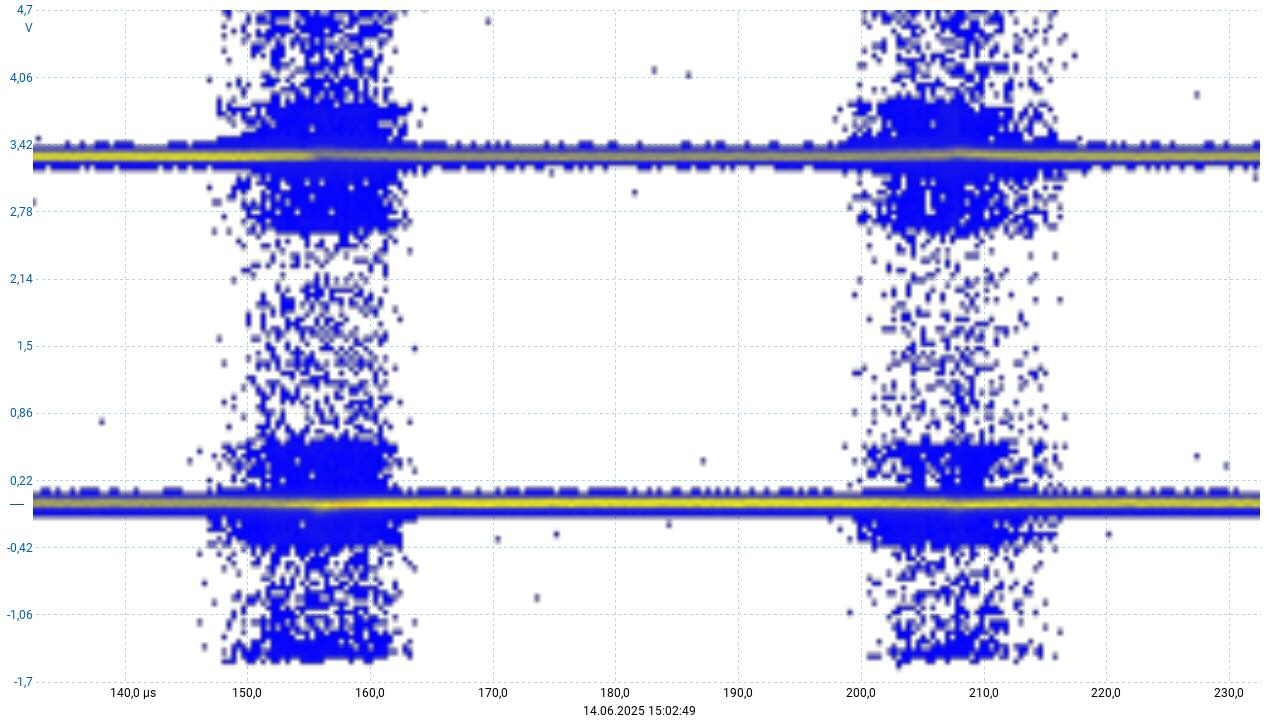
\includegraphics[width=1\textwidth]{fig/eye/eye_19200_15cm-zoom.jpg}
        \caption{Two-LEDs at 15cm}
        \label{fig:5.16-c}
    \end{subfigure}
    \hfill
    \begin{subfigure}[t]{0.48\textwidth}
        \centering
        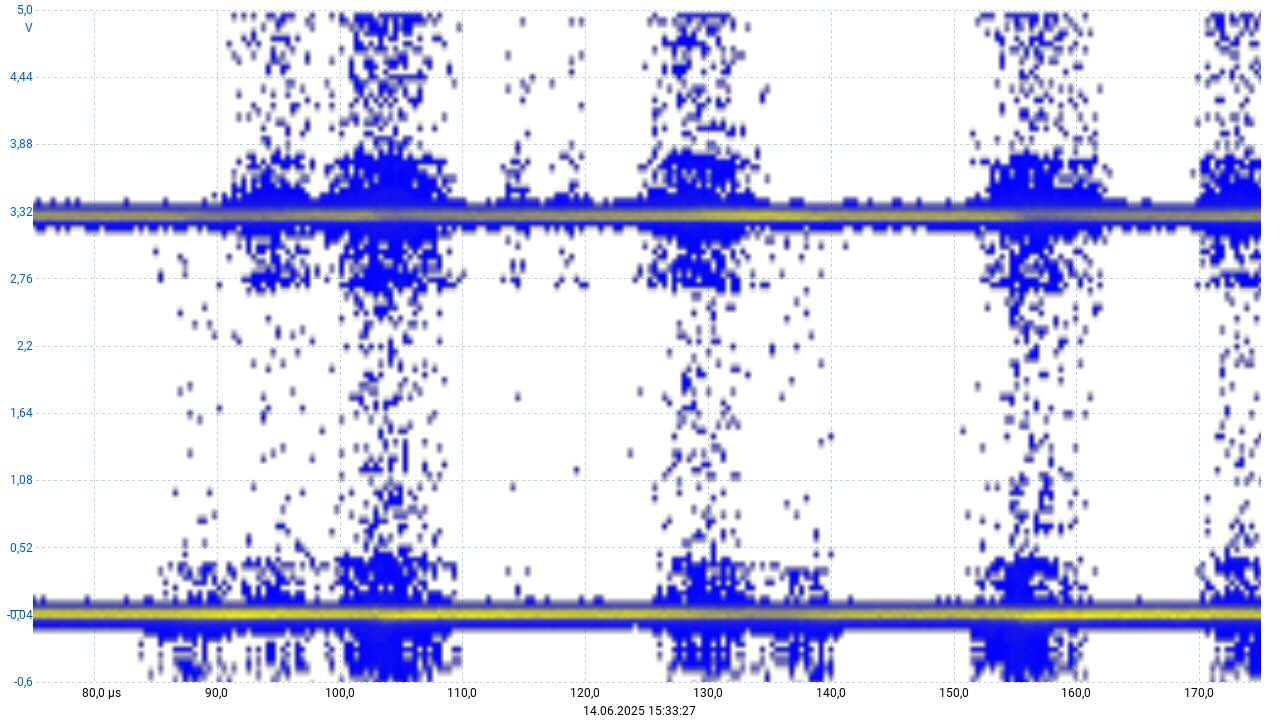
\includegraphics[width=1\textwidth]{fig/eye/eye_19200_5Led_15cm-zoom.jpg}
        \caption{Five-LEDs at 15cm}
        \label{fig:5.16-d}
    \end{subfigure}

    \caption{Eye diagram of 19200 baud rate at different distances and configurations}
    \label{fig:5.16}
\end{figure}

\subsection{Demodulated Data}
An OOK-modulated Message sent from the Raspberry Pi is demodulated at the receiver end by the STM32 board. The demodulated message is checked for different Baud rates and distances in this part of the evaluation.

An example message, "helloworld," is sent from the Pico board. The number of LEDs is two. At first, the distance between the transmitter and the Receiver is kept at 5cm. The baud rate changed gradually from 2400 to 38400. The baud rate of STM32 also changed in the code. It was found that a lower baud rate could decode the message, but a higher baud rate above 19200 could not. At a 10cm distance, when baud rates are lower than 2400, the message can't be decoded. However, now it can be decoded up to 38400. At a 15 cm distance, baud rates lower than 4800 can't be decoded anymore. Findings are summarized in the Table \ref{tab:5.1}, where "+" means it can decode, "-" means it can't, and "/" means partial decoding capability:

\begin{table}
    \centering
    \caption{Effect of Baudrate and Distance on Demodulation}
    \begin{tabular}{|c|c|c|c|}
    \hline
         \textbf{Baudrate} &\textbf{5cm}  &\textbf{10cm}  &\textbf{15cm} \\
         \hline
         2400 &+  &/  &/ \\
         \hline
         4800 &+  &+  &/ \\
         \hline
         9600 &+  &+  &+ \\
         \hline
         14400 &+  &+  &+ \\
         \hline
         19200 &/  &+  &+ \\
         \hline
         28800 &-  &+  &+ \\
         \hline
         38400 &-  &+  &+ \\
         \hline
    \end{tabular}
    \label{tab:5.1}
\end{table}

The Demodulated Data by the serial decoder at different Baud rates at 15cm is shown in Figure \ref{fig:5.15}. It again indicates that a 15cm baud rate of 4800 is not suitable, as only the starting bits can be demodulated. For other baud rates, demodulation at 15 cm is appropriate.

\begin{figure}[t]
    \centering
    
    % First row of subfigures
    \begin{subfigure}[t]{0.48\textwidth}
        \centering
        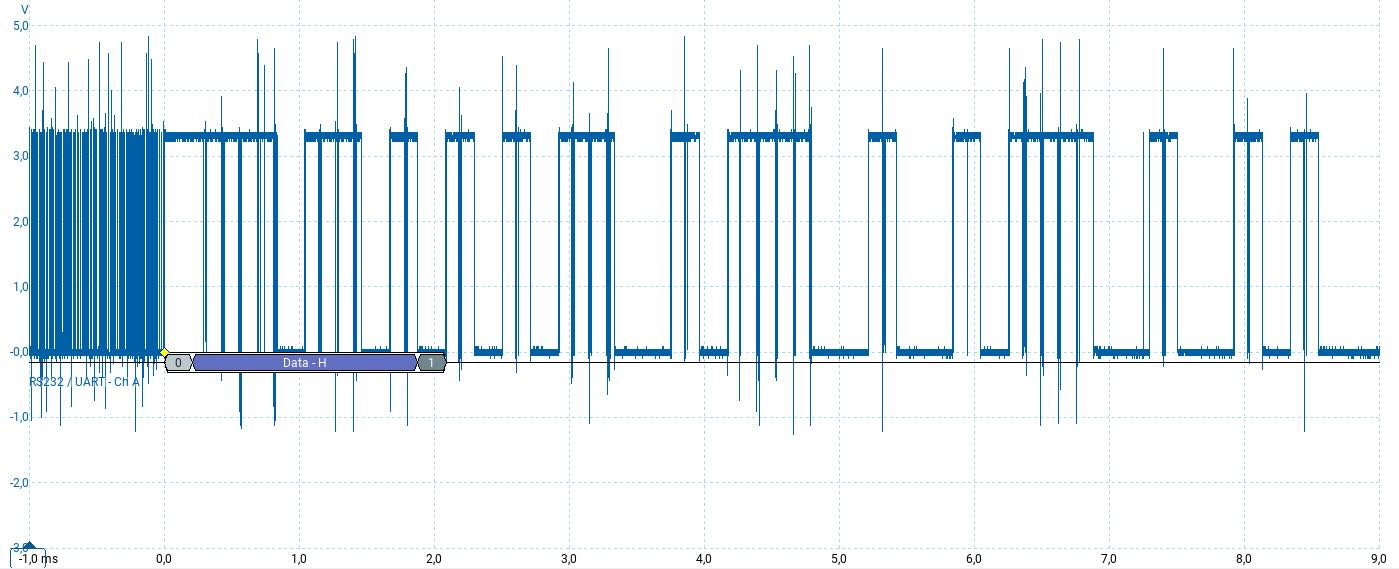
\includegraphics[width=1\textwidth]{fig/demod/Demod_4800_15cm.jpg}
        \caption{Baud rate 4800}
        \label{fig:5.17-a}
    \end{subfigure}
    \hfill
    \begin{subfigure}[t]{0.48\textwidth}
        \centering
        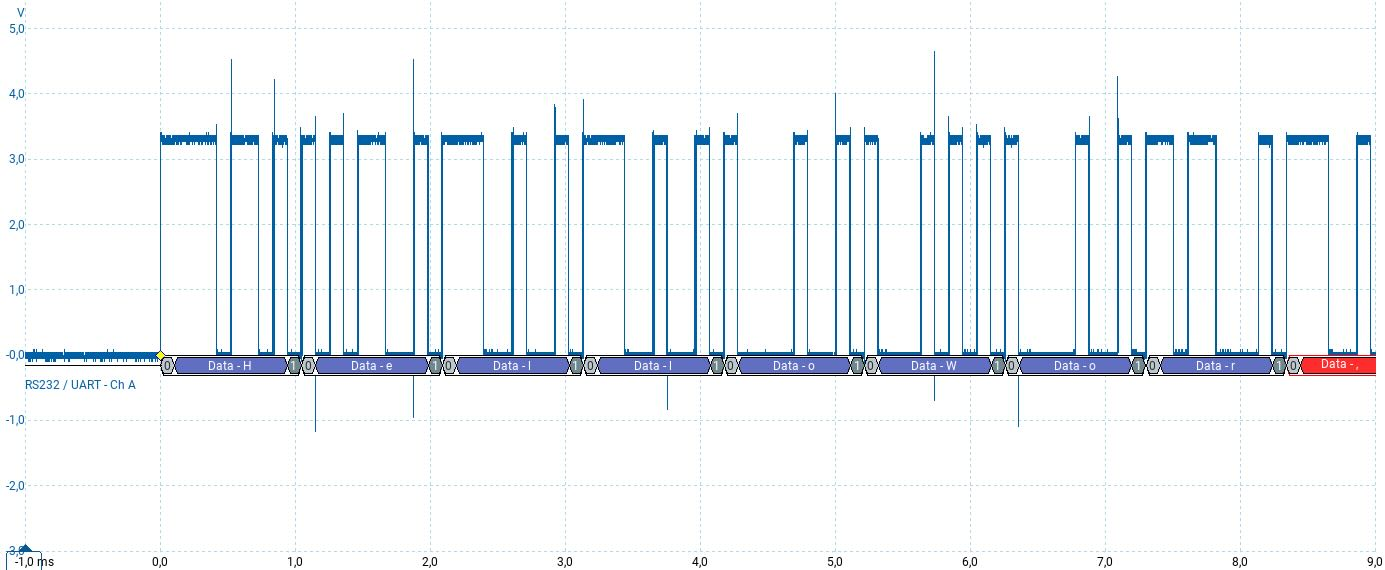
\includegraphics[width=1\textwidth]{fig/demod/Demod_9600_15cm.jpg}
        \caption{Baud rate 9600}
        \label{fig:5.17-b}
    \end{subfigure}
    
    \vspace{0.5em} % Small vertical space between rows

    % Second row of subfigures
    \begin{subfigure}[t]{0.48\textwidth}
        \centering
        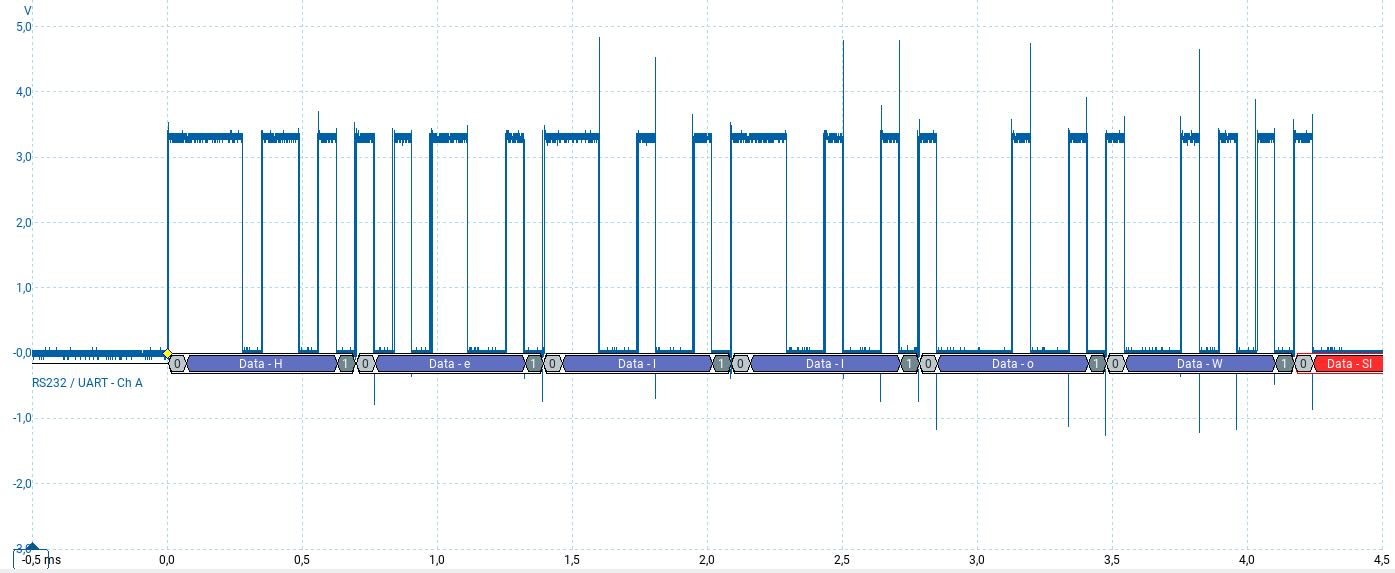
\includegraphics[width=1\textwidth]{fig/demod/Demod_14400_15cm.jpg}
        \caption{Baud rate 14400}
        \label{fig:5.17-c}
    \end{subfigure}
    \hfill
    \begin{subfigure}[t]{0.48\textwidth}
        \centering
        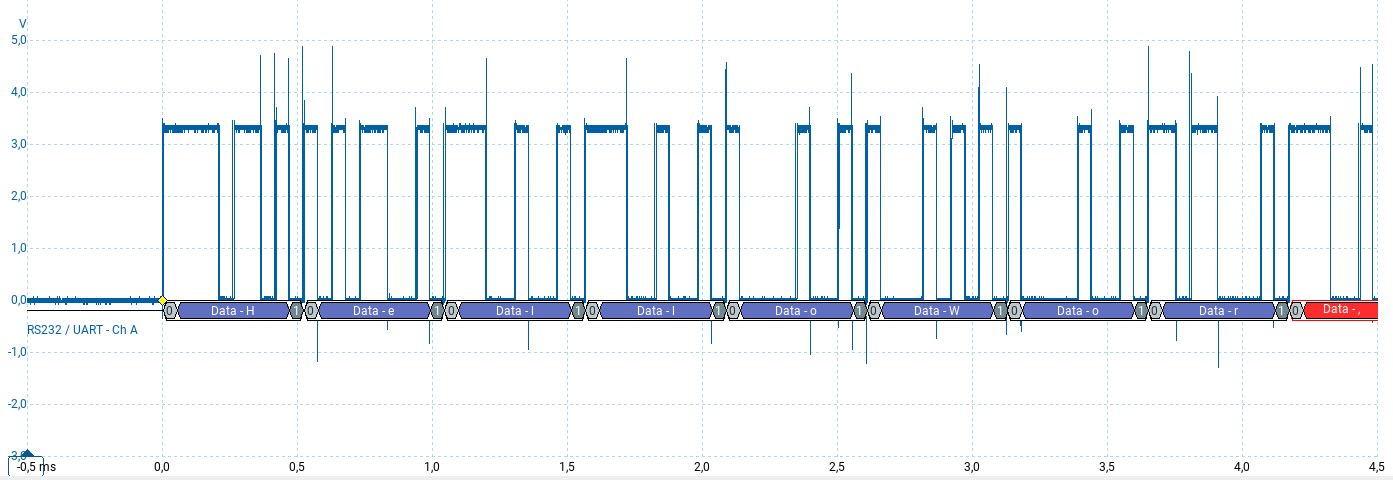
\includegraphics[width=1\textwidth]{fig/demod/Demodulated 19200_15cm.jpg}
        \caption{Baud rate 19200}
        \label{fig:5.17-d}
    \end{subfigure}

    \caption{Demodulated Data at different Baud rates at 15cm}
    \label{fig:5.17}
\end{figure}

This thesis also checked the possibilities of using five LEDs instead of two and demodulated the sent data. Baudrate varied from 9600 to 19200 at 10 and 15cm. The results are shown in the Table \ref{tab:5.2}.
Considering the result in the Table \ref{tab:5.1} and \ref{tab:5.2}, Baud rates 9600 and 14400 are the most suitable for data communication for this particular circuit at variable distances. 

\begin{table}
    \centering
    \caption{Effect of Baudrate, Diatance on Demodulation(5LEDs)}
    \begin{tabular}{|c|c|c|}
    \hline
         \textbf{Baudrate} &\textbf{10cm}  &\textbf{15cm} \\
         \hline
         9600 &/  &+   \\
         \hline
         14400 &/  &+   \\
         \hline
         19200 &-  &-   \\
         \hline
    \end{tabular}
    \label{tab:5.2}
\end{table}



\section{Energy Harvesting}

A \ac{EH} unit must check the time necessary to charge and discharge its battery or supercapacitor, depending on various conditions \cite{de2024reconfigurable}. Paper \cite{fong2012integrated} checked the amount of charge stored depending on battery energy density and its charge-discharge time. It also compared the power generated and the energy stored, and generated power vs distance \cite{fong2012integrated}.

In this subsection, the energy consumption of the communication branch will be discussed first. Then, the energy harvested by the Photodiodes and the Solar panel will be addressed. Later, the performance of the \ac{EVM} and supercapacitor charging and discharging will be shown.

\subsection{Energy Consumption}

The communication branch's power consumption is measured along with its voltage and current. When the STM32 board runs in regular (decoding) mode, it consumes between 5.3mA and 7.8mA at rated 3.3V. The TIA and comparator circuit's current consumption is 3.7mA to 4.2mA. This results in a total current consumption of the communication branch at a rated 3.3V of 0.009 to 0.012A. So, the total power consumption of the communication at regular decoding mode is between 0.030 and 0 .036W.

In power-saving mode (STOP Mode), STM32 consumes only 0.113mA, which makes the communication branch's current consumption 0.003A. The TIA and comparator circuit's current consumption is  \(\sim\) 3mA. Thus, the communication branch's total power consumption becomes only 0.010W. Findings are shown in the Table \ref{tab:5.3}.

\begin{table}
    \centering
    \caption{Voltage, Current, and Power Consumption of Receiver circuit}
    \begin{tabular}{|c|c|c|}
    \hline
         \textbf{parameter} &\textbf{Decoding Mode}  &\textbf{STOP Mode} \\
         \hline
         Voltage &3.3V  &3.3V   \\
         \hline
         Current &5.3mA to 7.8mA &3mA   \\
         \hline
         Power &.03 to .036W  &.010W   \\
         \hline
    \end{tabular}
    \label{tab:5.3}
\end{table}

\subsection{Energy Harvested}

At first, light from one LED was projected on nine \ac{PD}s connected in series, as in Figure \ref{fig:4.3}, in a confined box, and the distance between the LED and the \ac{PD}s was kept at 5cm. The voltage output from the \ac{PD}s is 1.79V, which is well above the cold start voltage, but the current generated is too small, even below .5\(\mu\)A. This can not start the booster circuit, hence it can't charge the supercapacitor or give an output. 


As more current is necessary to operate the \ac{EVM}, the new configuration of the \ac{PD} was tried out, as in Figure \ref{fig:4.6}. The output current from \ac{PD}s is 1.2 \(\mu\)A, and the voltage is 0.65V. Now the power is 0.00078 mW, more than before at 5cm. But it can neither do a cold start of the \ac{EVM} nor run the circuit in regular condition(booster charger is above 1.8 typical). Using Solar Panel instead of \ac{PD}s, current is found 13\(\mu\)A and voltage 1.15V. The produced power is 0.014mW, below the minimum cold input power of 0.015mW, but is more than the minimum input power (.005mW) for regular charging. This indicates that adding a partially charged capacitor can run in regular conditions. Later, two-LED and five-LED configurations were used, and the power generation was measured. The effect of distances on \ac{EH} is shown in Figure \ref{fig:5.18}. A 60W bulb is also held at a 5cm distance from the photodiodes configuration and the solar panel to see the highest possible energy harvest capability. The highest energy that can be produced for each configuration is 0.0015W and .0549W, respectively.

\begin{figure}[t]
    \centering
    
    % First row of subfigures
    \begin{subfigure}[t]{0.48\textwidth}
        \centering
        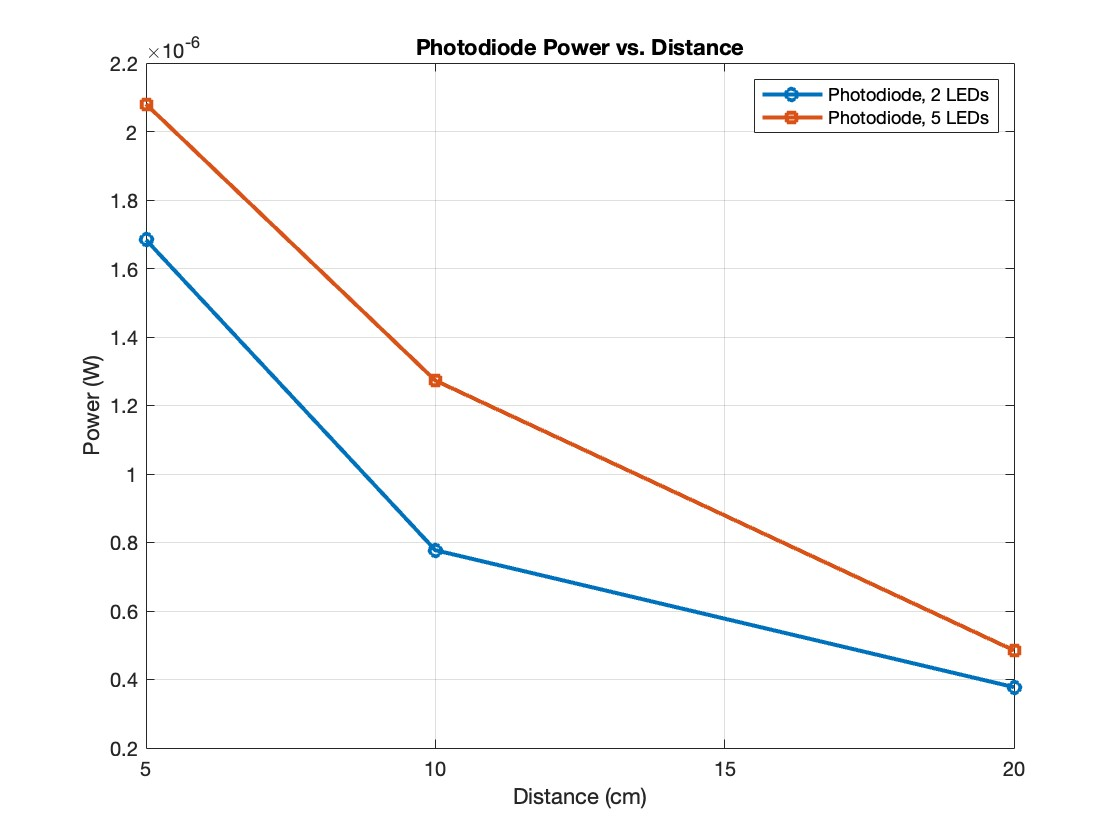
\includegraphics[width=1\textwidth]{fig/energy_photodiode.jpg}
        \caption{Photodiodes}
        \label{fig:5.18-a}
    \end{subfigure}
    \hfill
    \begin{subfigure}[t]{0.48\textwidth}
        \centering
        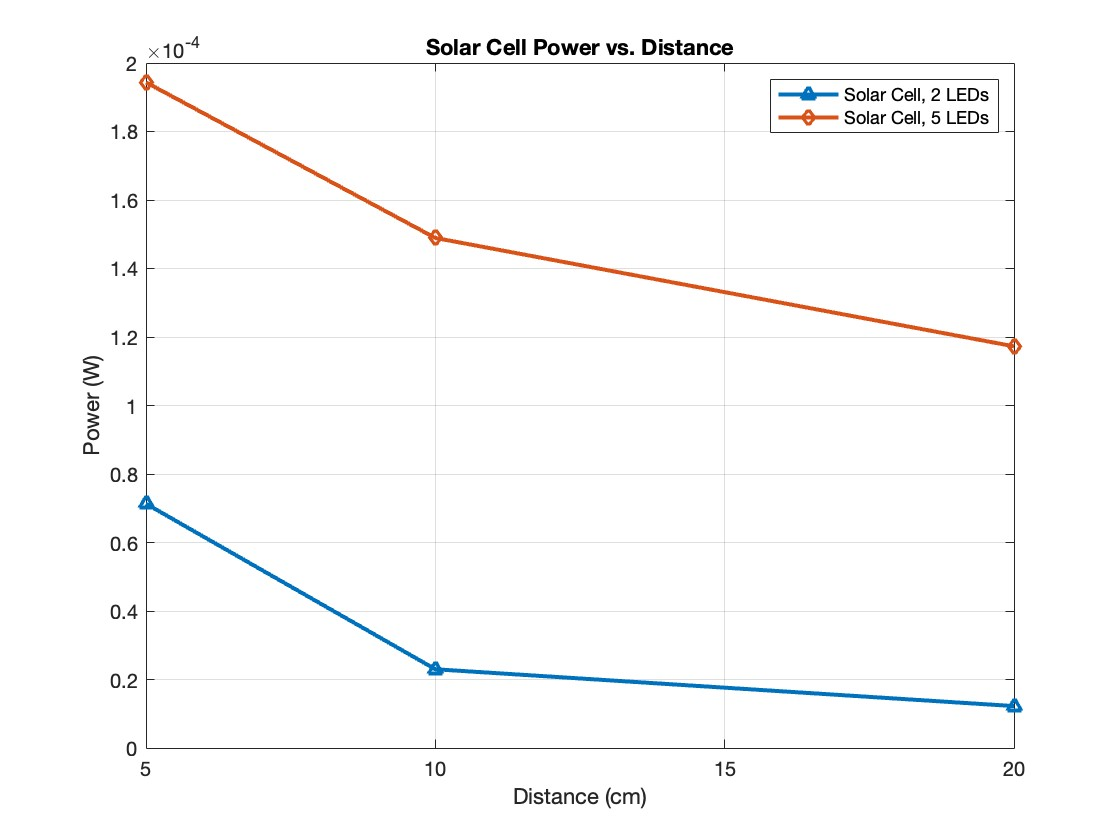
\includegraphics[width=1\textwidth]{fig/energy_solar.jpg}
        \caption{Solar Panel}
        \label{fig:5.18-b}
    \end{subfigure}

    \caption{Power generation by Photodiodes and Solar Panel vs distances}
    \label{fig:5.18}
\end{figure}


\subsection{Performance of the EVM and Supercapacitor}

At first, the supercapacitor was tried to be charged using 2 LEDs for both Photodiodes and a Solar panel. When a partially charged supercapacitor is attached, the boost charger can harvest power from a low voltage source\cite{slusbh2}. This thesis does this to avoid a cold start and a long waiting period.

With a partially charged supercapacitor, two LEDs, and the \ac{PD}s connected, the load discharged the supercapacitor to 2.8 in 44.6 seconds. Once discharged to the undervoltage protection level, the voltage at the output switched to near zero (\(\sim\)0.5 V). The supercapacitor started charging again, but it stuck at 3.2V, which means it could not go above the battery's Hysterisis level with the load connected and provide any power to the load. This is shown in the Figure \ref{fig:5.19}. From now on, in every figure, the blue line represents supercapacitor voltage, and the red line shows voltage output from \ac{EVM}. Similarities are observed when a Solar panel uses a partially charged supercapacitor and two LEDs. Now it takes 49 seconds to discharge the supercapacitor to 3.2 and make \ac{EVM} go to 0.5V, as shown in the Figure \ref{fig:5.20}.

\begin{figure}
    \centering
    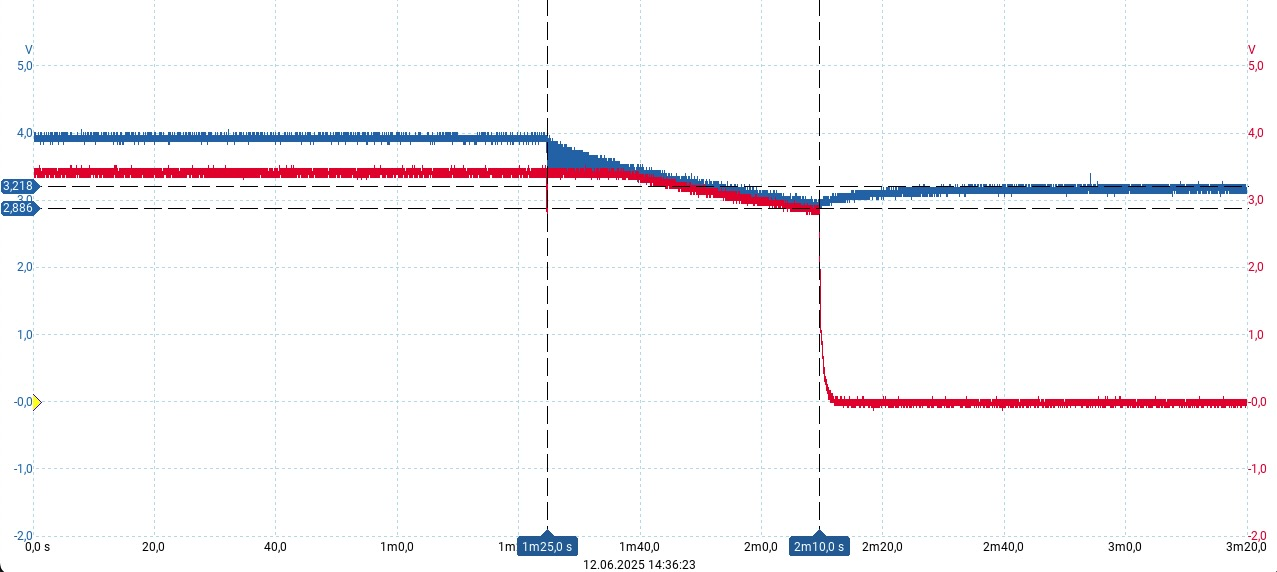
\includegraphics[width=0.75\linewidth]{fig/Supercap_2L_Photodiode_pre.jpg}
    \caption{Supercapacitor and EVM output voltage when light fed from 2 LED to Photodiodes}
    \label{fig:5.19}
\end{figure}

\begin{figure}
    \centering
    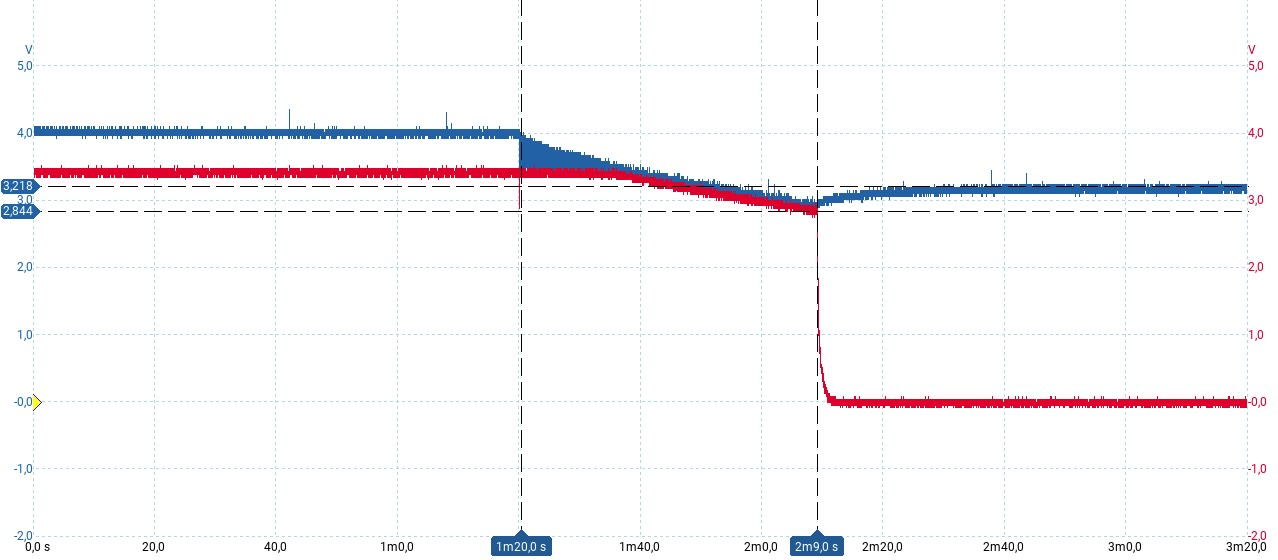
\includegraphics[width=0.75\linewidth]{fig/Supercap_Vout_2L_Solar_Pre.jpg}
    \caption{Supercapacitor and EVM output voltage when light fed from 2 LED to Solar Panel.}
    \label{fig:5.20}
\end{figure}

To evaluate the best possible performance of \ac{EVM} under maximum light exposure conditions, a 60W light is used. Even with 60W light, photodiodes still require more than 40 minutes to charge the supercapacitor above 3.2V. This is also observed in the paper \cite{de2024reconfigurable} to be around 32min. A partially charged supercapacitor can be added to reduce time, as explained in \cite{slusbh2}. Photodiodes maintain a voltage of 4.5V when there is no load, as shown in Figure \ref{fig:5.21}. However, it discharges within 92 seconds when a load is connected.

\begin{figure}
    \centering
    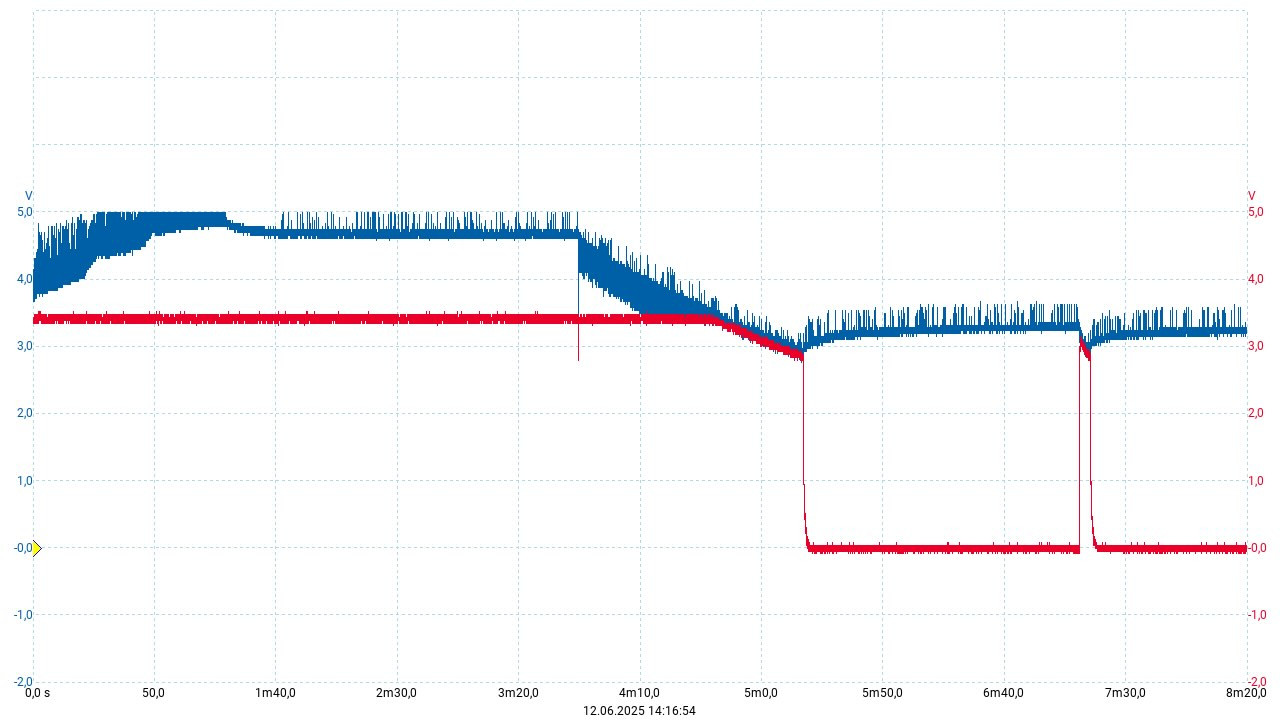
\includegraphics[width=0.75\linewidth]{fig/supercap_Vout_60w_light-photodiode_precharged.jpg}
    \caption{EVM performance when Photodiodes under 60W and supercapacitor precharged.}
    \label{fig:5.21}
\end{figure}


It took a solar panel 2 minutes and 45 seconds to fully charge the supercapacitor under 60W light, shown in \ref{fig:5.22}. When light was still shining, spikes were shown in the blue line. This is because it was trying to reach its highest permitted voltage of 5.1V. When the light was switched off, the line became more stable and maintained a voltage of 4.5V. The voltage output drops near zero when the load is connected somewhere near 7 seconds. \ac{EVM} tried to charge the supercapacitor again multiple times. When it charged more than 3.2, it tried to supply voltage to Vout but failed, as evident in the Figure \ref{fig:5.22}. When the load is connected to the \ac{EVM} from the start, shown in Figure \ref{fig:5.23}. The \ac{EVM} tried to charge up the supercapacitor and give Vout a couple of times, shown as spikes.

\begin{figure}
    \centering
    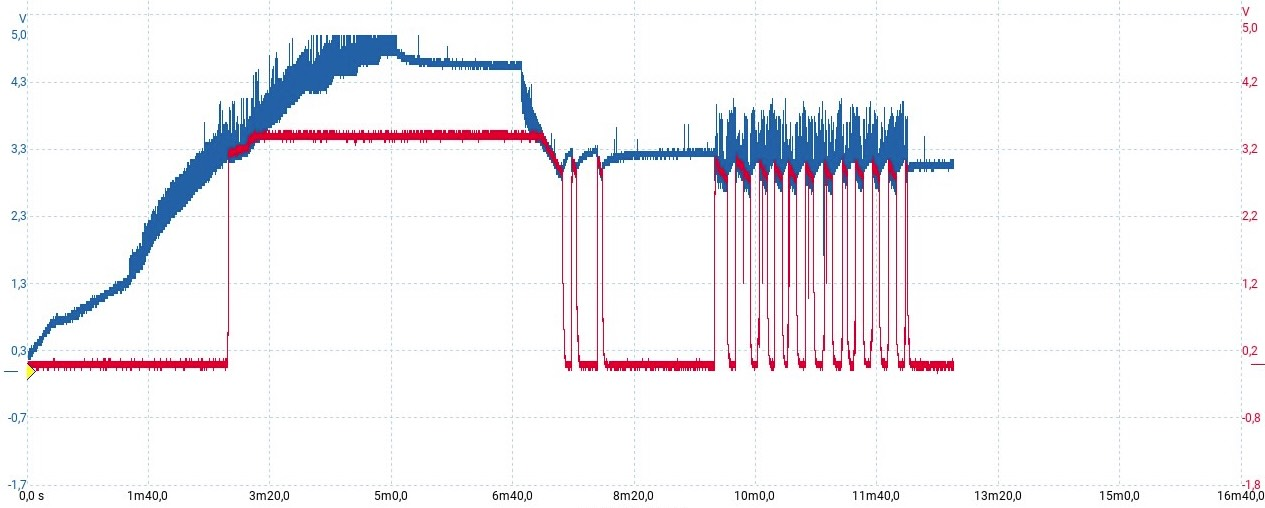
\includegraphics[width=0.75\linewidth]{fig/60W_solar.jpg}
    \caption{EVM performance when Solar Panel under 60W}
    \label{fig:5.22}
\end{figure}



\begin{figure}
    \centering
    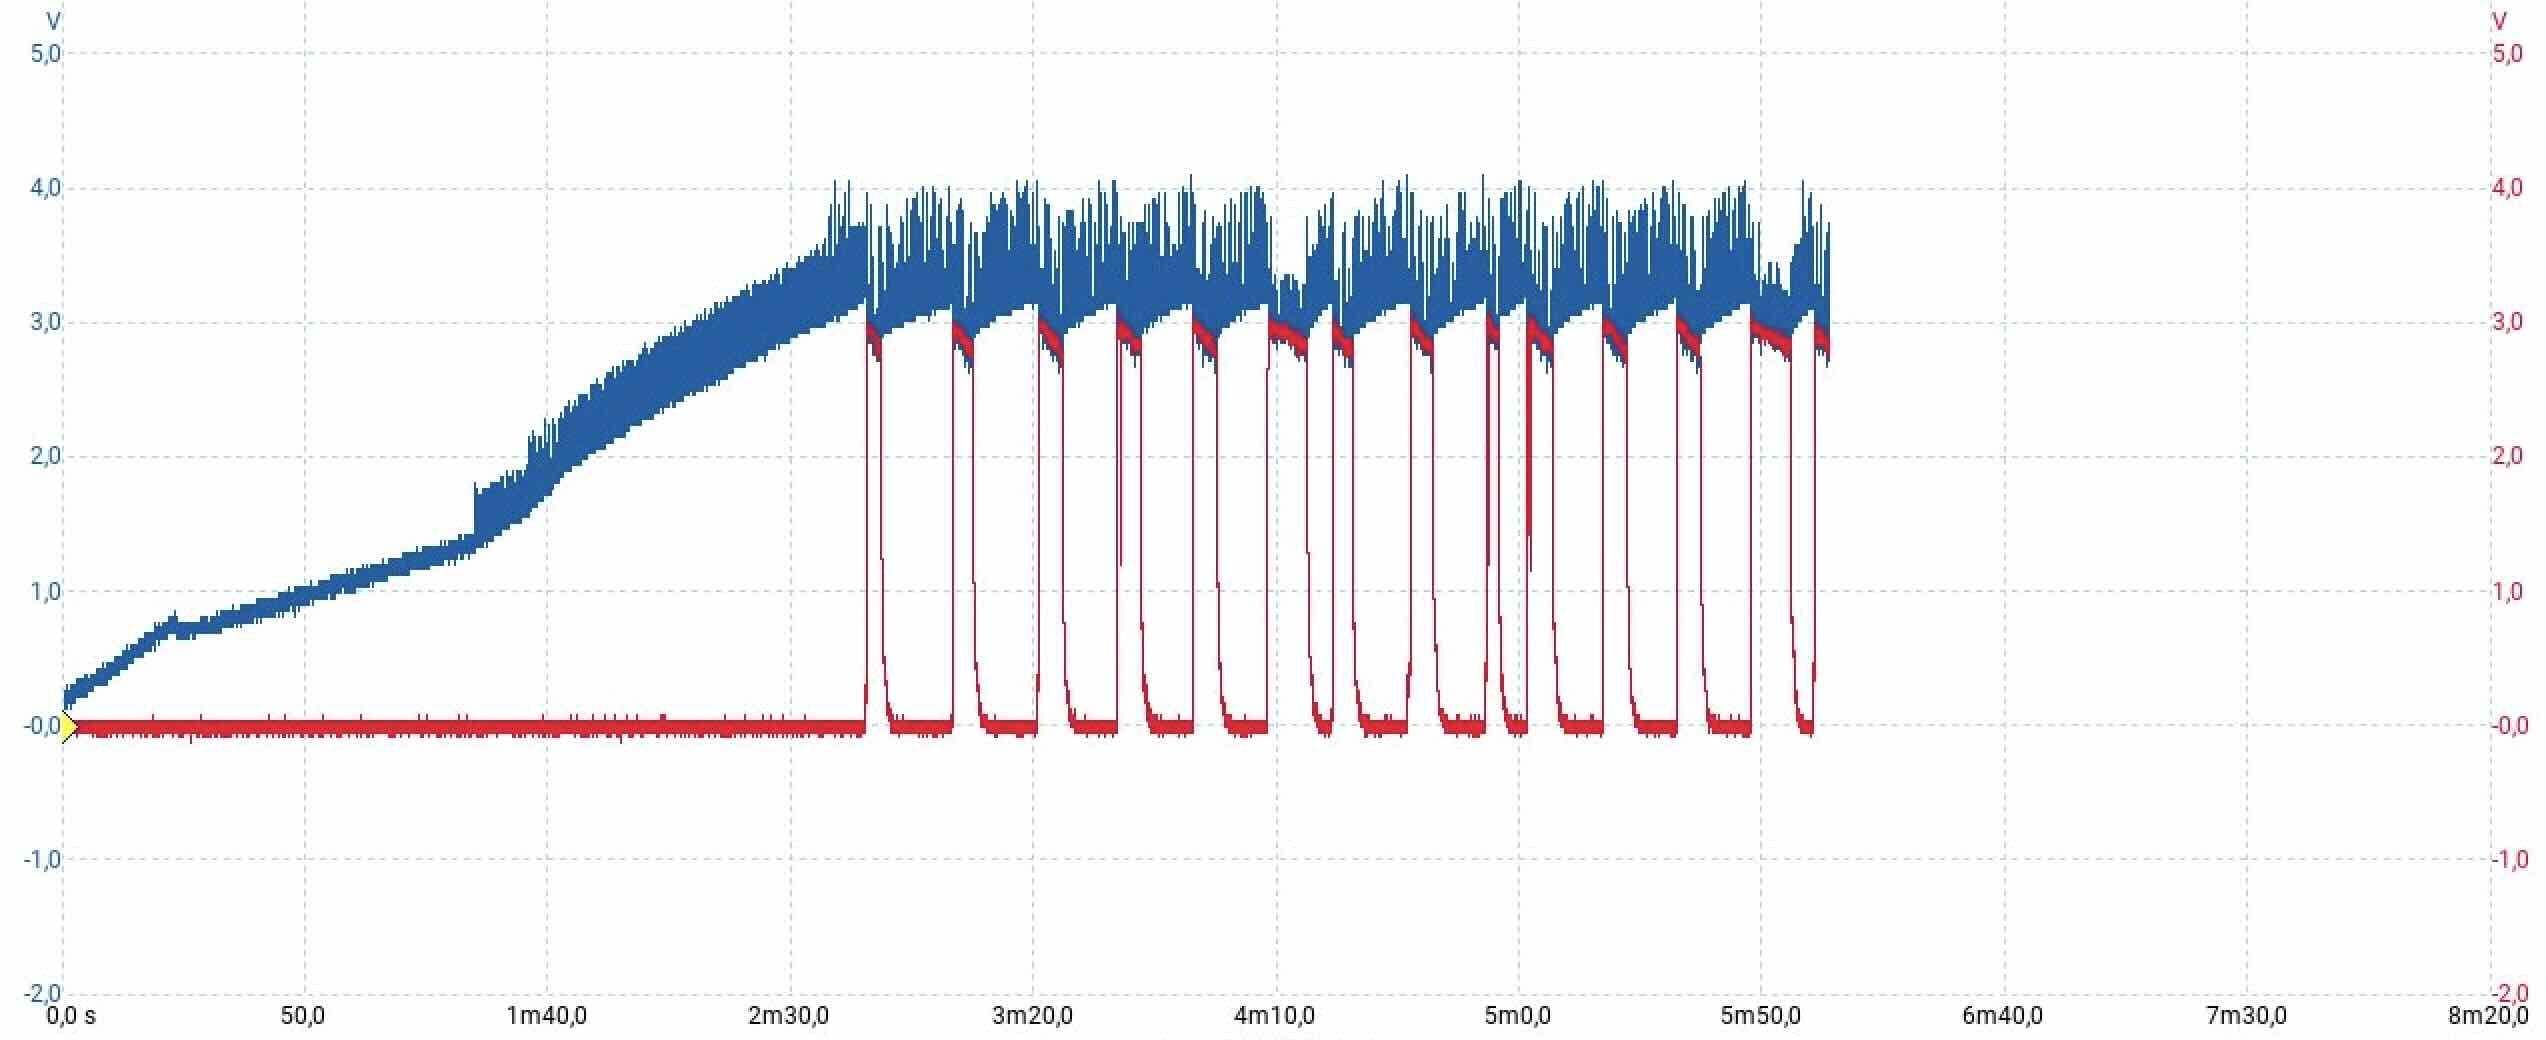
\includegraphics[width=0.75\linewidth]{fig/60W_solar_load.jpg}
    \caption{EVM performance when Solar Panel under 60W connected to load connected from start}
    \label{fig:5.23}
\end{figure}

An attempt was also made to use a 1F supercapacitor instead of a 0.1F to see the effect. As shown in the Figure \ref{fig:5.24}, it took 6 minutes and 45 seconds to charge it to more than 3.2 volts and have a Vout from \ac{EVM}. However, this didn't improve the voltage drop condition once the load was connected as shown in Figure \ref{fig:5.25}.

\begin{figure}
    \centering
    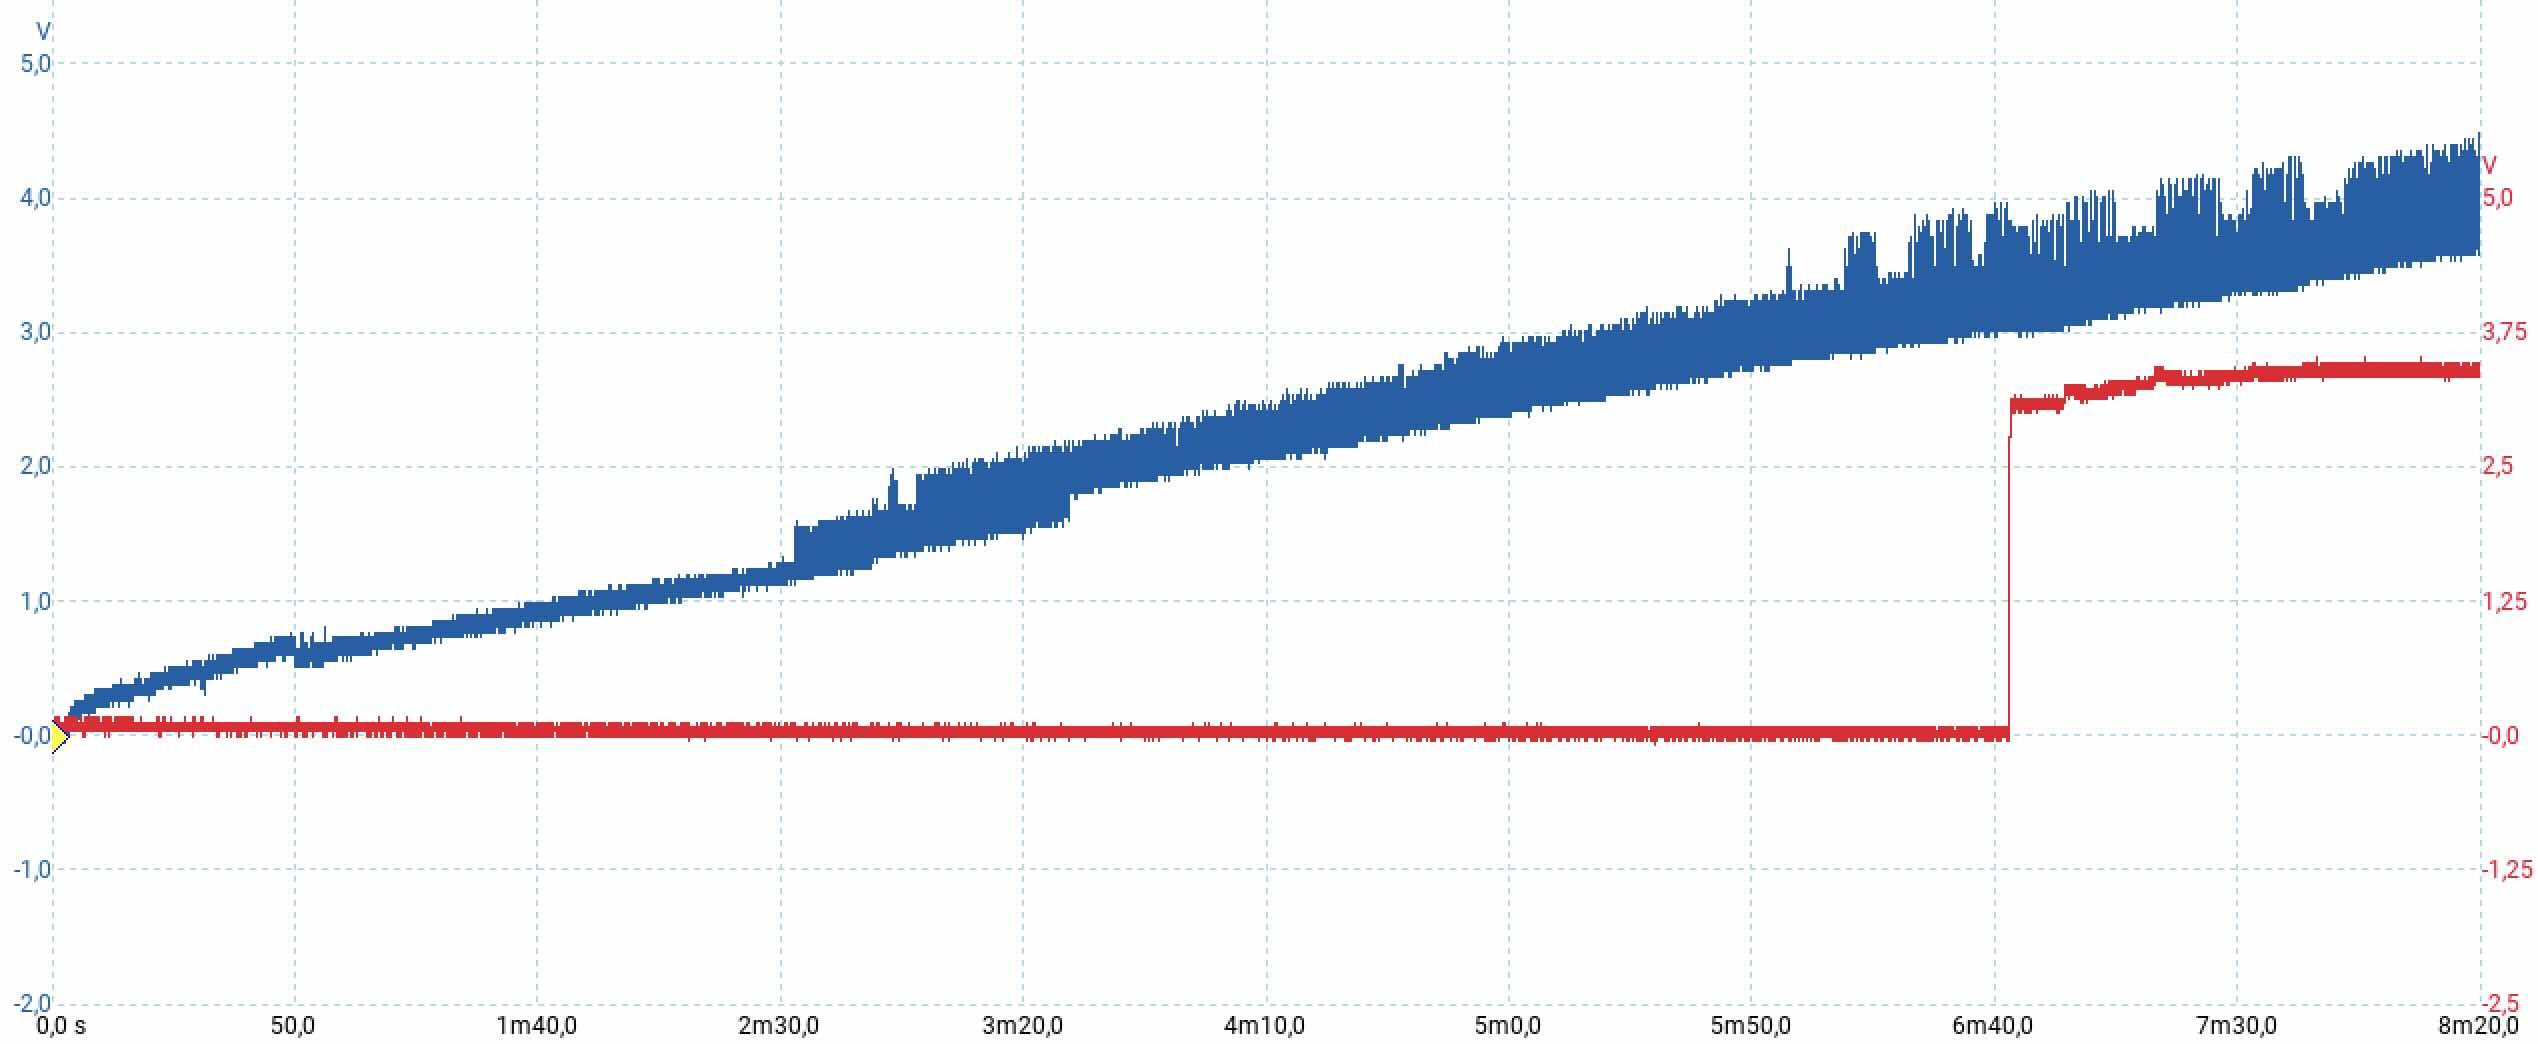
\includegraphics[width=0.75\linewidth]{fig/1F_supercap_charging_Solar_60w.jpg}
    \caption{Enter Caption}
    \label{fig:5.24}
\end{figure}

\begin{figure}
    \centering
    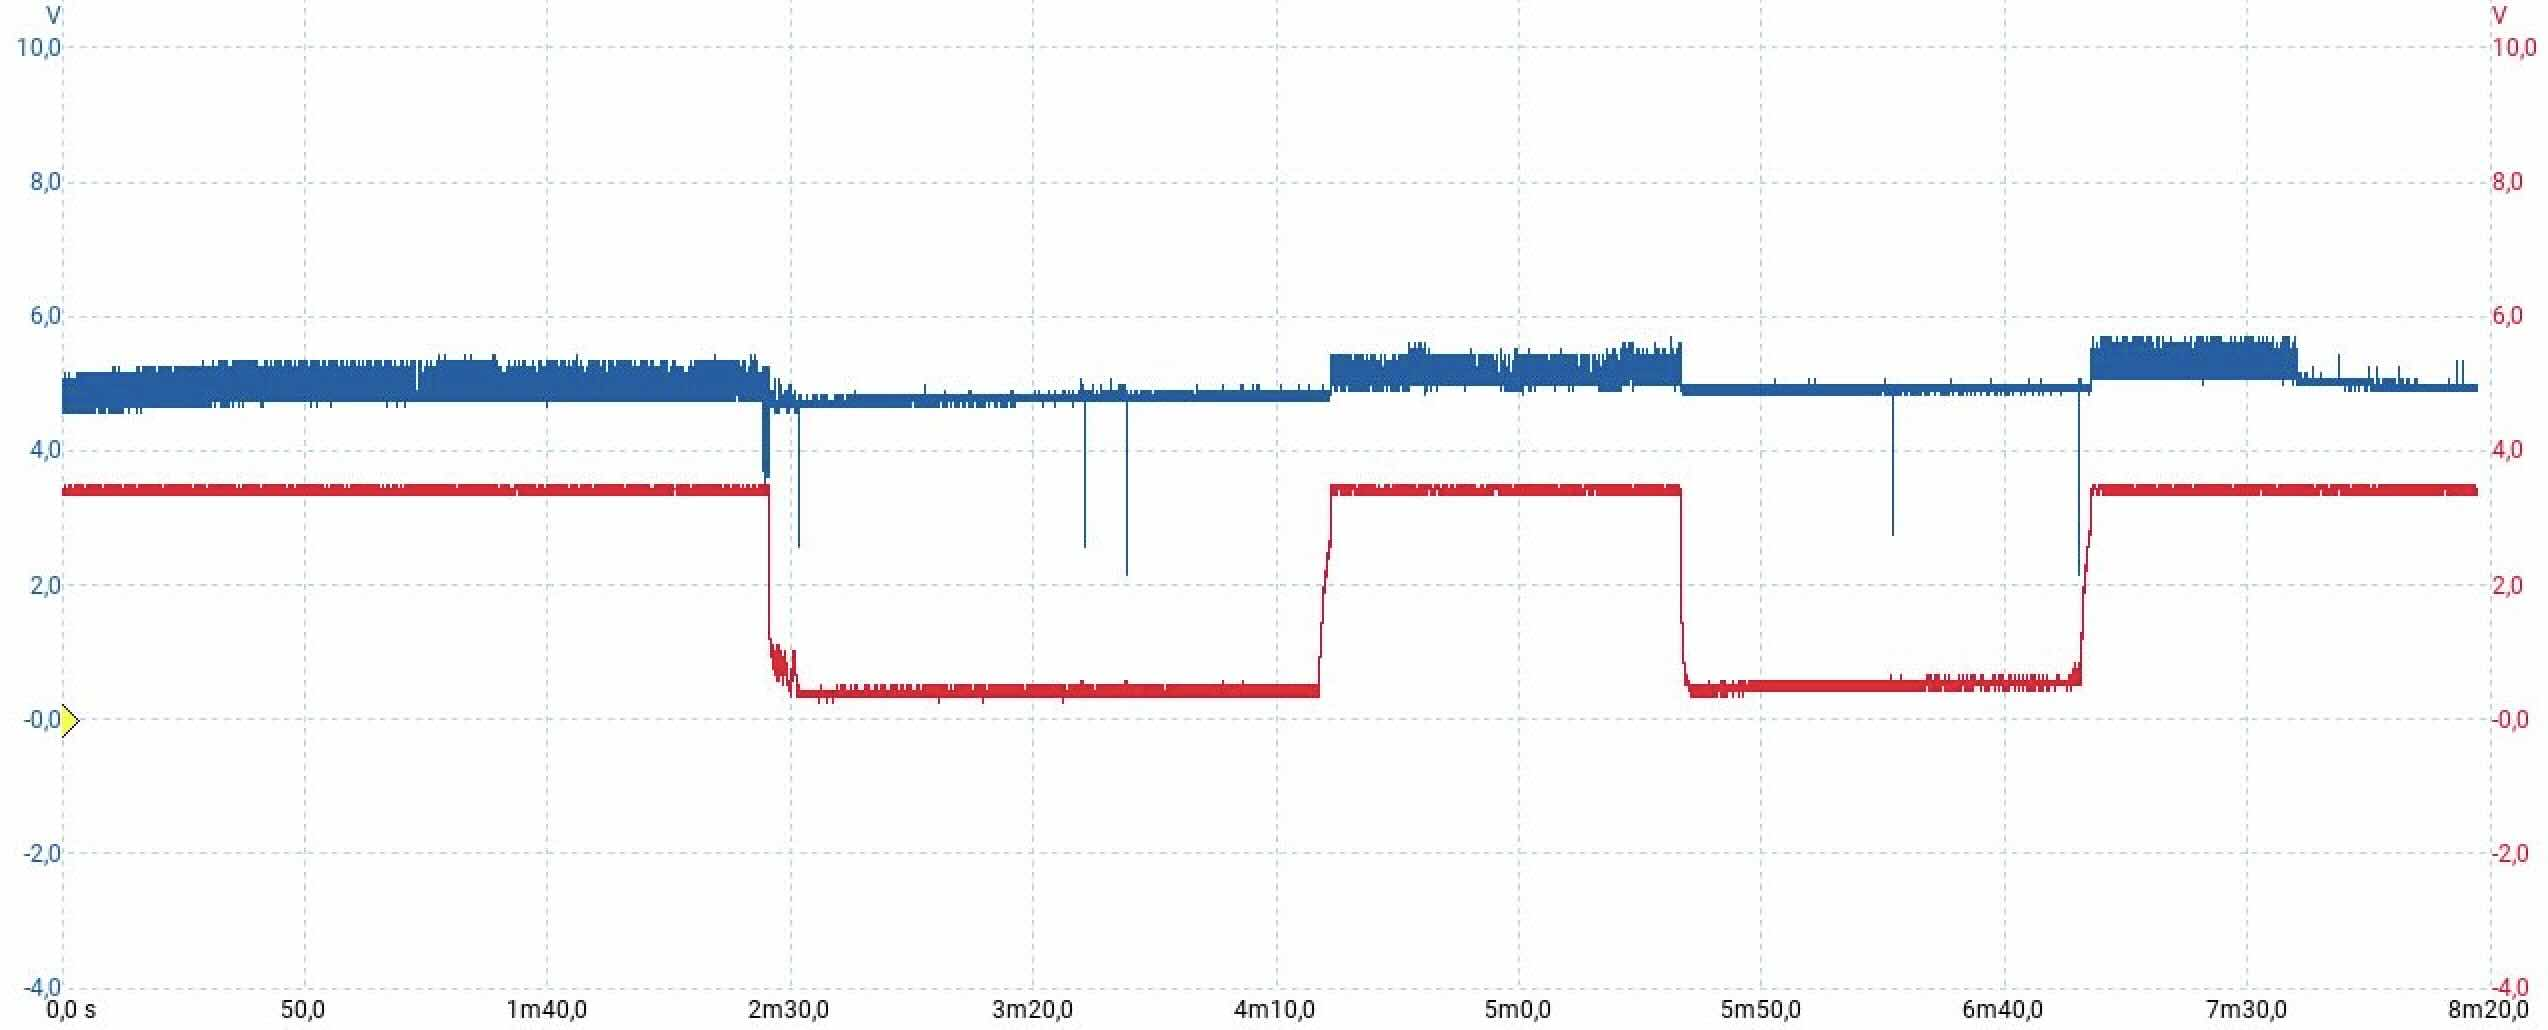
\includegraphics[width=0.75\linewidth]{fig/60W_solar_pre_1F.jpg}
    \caption{EVM performance when Solar Panel under 60W and Supercapacitor 1F}
    \label{fig:5.25}
\end{figure}





